\documentclass{article}
\usepackage[utf8]{inputenc}
\usepackage[spanish]{babel}
\usepackage{hyperref}
\usepackage[pdftex]{graphicx}
\usepackage{float}
\usepackage[top=1.5in, bottom=1.5in, left=1in, right=1in]{geometry}
\newcommand{\HRule}{\rule{\linewidth}{0.5mm}}
\usepackage{listings}
\lstloadlanguages{C++}
\lstnewenvironment{code}
	{%\lstset{	numbers=none, frame=lines, basicstyle=\small\ttfamily, }%
	 \csname lst@SetFirstLabel\endcsname}
	{\csname lst@SaveFirstLabel\endcsname}
\lstset{% general command to set parameter(s)
	language=C++, basicstyle=\small\ttfamily, keywordstyle=\slshape,
	basewidth={0.47em,0.40em},
	columns=fixed, fontadjust, resetmargins, xrightmargin=5pt, xleftmargin=15pt,
	flexiblecolumns=false, tabsize=2, breaklines,	breakatwhitespace=false, extendedchars=true,
	numbers=left, numberstyle=\tiny, stepnumber=1, numbersep=9pt,
	frame=l, framesep=3pt,
}
\lstset{
     literate=%
         {á}{{\'a}}1
         {é}{{\'e}}1
         {í}{{\'i}}1
         {ó}{{\'o}}1
         {ú}{{\'u}}1
         {Á}{{\'A}}1
         {É}{{\'E}}1
         {Í}{{\'I}}1
         {Ó}{{\'O}}1
         {Ú}{{\'U}}1
         {ñ}{{\v{n}}}1
         {Ñ}{{\v{N}}}1
}

\begin{document}

\pagenumbering{Alph} %linea dummy solo para evitarme un warning
\begin{titlepage}
\begin{center}


\includegraphics[width=0.35\textwidth]{logo_uba}\\[1cm]

\textsc{\LARGE Departamento de Computaci\'on}\\[1.5cm]

\textsc{\Large Facultad de Ciencias Exactas y Naturales}\\[0.5cm]
\textsc{\Large Universidad de Buenos Aires}\\[0.5cm]

% Title
\HRule \\[0.4cm]
{ \huge \bfseries Sistemas Operativos \\[0.4cm] }

\HRule \\[1.5cm]

% Author
\emph{Autor:}\\
Leopoldo \textsc{Taravilse}

~

\emph{Corrección y extensión:}\\
Roberto \textsc{Rama}

\vfill

% Bottom of the page
\emph{Última fecha de edición:}\\
{\large \today}

\end{center}
\end{titlepage}
\pagenumbering{arabic}
\tableofcontents
\newpage
\section{Procesos}

\subsection{¿Qu\'e es un proceso?}

Un proceso es un programa en ejecuci\'on. El proceso incluye no s\'olo el c\'odigo del programa sino tambi\'en el estado de los registros, la memoria que utiliza el proceso y todos los dem\'as recursos que utiliza durante su ejecuci\'on.

Un proceso tiene cinco posibles estados:
\begin{itemize}
\item New: El estado del proceso mientras est\'a siendo creado.
\item Ready: El estado del proceso que est\'a listo para correr y a la espera de un procesador para correr.
\item Running: El estado del proceso que est\'a actualmente corriendo. Puede haber s\'olo un proceso en estado running al mismo tiempo.
\item Waiting: El estado del proceso cuando est\'a esperando un evento como puede ser entrada/salida.
\item Terminated: El estado del proceso cuando ya finaliz\'o su ejecuci\'on.
\end{itemize}

Todos los procesos est\'an representados en el sistema operativos por su \textbf{Process Control Block (PCB)}. La PCB almacena entre otras cosas
\begin{itemize}
\item El estado del proceso.
\item El Program Counter asociado a ese proceso, que indica cu\'al es la pr\'oxima instrucci\'on a ejecutar.
\item El estado de los registros de la CPU asociados al proceso.
\item Informaci\'on sobre la memoria asociada al proceso.
\item Informaci\'on de entrada/salida. Esto incluye por ejemplo la lista de archivos abiertos o de dispositivos de entrada/salida con los que interactua el proceso.
\end{itemize}

Cada proceso es un\'ivocamente identificado por su \textbf{pid (process id)}.

\subsection{Creando procesos}

Un proceso puede crear otros procesos. Si un proceso $A$ crea un proceso $B$ decimos que $A$ es el proceso padre, y $B$ es el proceso hijo.

En Linux para crear un proceso, el proceso padre debe llamar a la funci\'on $fork$, que es una system call. Luego de que la instrucci\'on $fork$ es ejecutada, dos procesos pasan a existir en lugar de uno. La forma de reconocer cu\'al es el proceso padre y cu\'al es el proceso hijo es mediante el valor de retorno de $fork$. Si al ejecutarse $fork$ retorna 0, eso quiere decir que el proceso es el hijo, si en cambio retorna un valor distinto de cero, el proceso es el padre y el valor de retorno es el pid del proceso hijo que se acaba de crear.

Cuando un proceso es creado, no necesariamente tiene que seguir ejecutando el c\'odigo del proceso padre. La funci\'on $exec$ (que tambi\'en es una system call), permite a un proceso (generalmente es el hijo quien la invoca) cambiar su c\'odigo por el de otro programa. Esto permite que un proceso cree otro proceso, para que ejecute el c\'odigo de otro programa.

Tambi\'en existe la system call $wait$, que le permite a un padre esperar a que termine la ejecuci\'on de su proceso hijo. Si el padre tuviese m\'as de un hijo, y se quisiera esperar a que terminen todos ellos, deber\'ia hacerse un $wait$ por cada uno de sus hijos.

Para terminar un proceso, existe la system call $exit$, que le indica a su padre que el proceso hijo ya ha finalizado su ejecuci\'on.

\subsection{Comunicaci\'on entre procesos}

En muchos casos es deseable que los procesos puedan comunicarse entre s\'i. Vamos a ver dos formas de comunicaci\'on entre procesos. Una de estas formas es mediante memoria compartida, mientras que la otra es el intercambio de mensajes entre procesos.

Para que los procesos se comuniquen mediante el uso de memoria compartida, estos deben avisarle al sistema operativo que compartir\'an parte de la memoria, ya que por defecto ning\'un proceso puede acceder a memoria que pertenece a otro proceso. Una vez que esto sucede, ambos procesos pueden leer y escribir en una misma regi\'on de la memoria, permitiendo que cada proceso pueda leer lo que el otro escribi\'o.

En Linux un espacio de memoria compartida se reserva mediante la system call $shmget$, mientras que se accede con la system call $shmat$. Para dejar de utilizar el espacio de memoria compartida se debe llamar a la system call $shmdt$ mientras que para liberar la memoria se utiliza la system call $shmctl$.

Para comunicar dos procesos mediante el intercambio de mensajes, se debe establecer una conexi\'on que permita dos operaciones b\'asicas: send y receive. Existen a su vez dos tipos de send y dos tipos de receive: bloqueante y no bloqueante. Un send bloqueante espera a que la otra parte reciba el mensaje, mientras que un receive bloqueante espera a que la otra parte envie el mensaje. En el caso del send y el receive no bloqueantes, simplemente hacen su tarea (enviar o recibir un mensaje) y el proceso sigue con su ejecuci\'on normalmente sin esperar nada del otro lado.

La implementaci\'on de Unix (y por lo tanto de Linux) del intercambio de mensajes es mediante sockets. Los sockets se pueden ver como extremos en una comunicaci\'on. Una vez creados los sockets, se puede escribir y leer como si fuesen un dispositivo de entrada/salida.

\section{Threads}

\subsection{¿Qu\'e es un thread?}

Hasta ahora estudiamos a los procesos como un \'unico hilo de ejecuci\'on que se ejecuta en una CPU. Los threads nos permiten separar los procesos en varios hilos de ejecuci\'on que pueden correr en simult\'aneo en distintas CPUs. Un thread es una unidad b\'asica de ejecuci\'on que tiene su propio \textbf{tid (thread id)}, que sirve para identificarlo de la misma manera que el pid identifica a un proceso, su propio estado del set de registros de la CPU, y su propia \'area de stack en memoria. Todos los dem\'as recursos como lo son por ejemplo la secci\'on de c\'odigo o datos en memoria, los archivos abiertos, o los dispositivos de entrada/salida con los que se comunica el thread, son compartidos con todos los threads del mismo proceso.

Algunas de las ventajas del uso de threads son:

\begin{itemize}
\item Cuando un proceso con un s\'olo thread est\'a a la espera de una operaci\'on bloqueante como puede ser la comunicaci\'on con un dispositivo de entrada/salida, un proceso con muchos threads puede tener un s\'olo thread bloqueado mientras que los dem\'as threads siguen ejecut\'andose sin tener que esperar.
\item Los threads de un mismo proceso comparten su memoria, por lo que es muy \'util crear threads en lugar de procesos cuando se quiere compartir memoria y c\'odigo.
\item Mientras que crear un proceso es muy costoso en t\'erminos de eficiencia, crear un thread es mucho m\'as econ\'omico, entre otras cosas porque no se tiene que reservar memoria o crear una PCB.
\item En arquitecturas con m\'ultiples procesadores el uso de threads permite la ejecuci\'on de un proceso en m\'as de una CPU, permitiendo as\'i que al correr distintos threads del mismo proceso en distintas CPUs, el proceso se ejecute m\'as r\'apido que un proceso monothread.
\end{itemize}

\subsection{Pthreads}

El standard de threads de POSIX, conocido como pthreads, define una API a la que se deben adaptarlas implementaciones de threads para sistemas operativos basados en Unix. El tipo de datos que se utiliza para crear threads es $pthread\_t$ y la forma decrear un thread es con la funci\'on $pthread\_create(\&tid,\&attr,startfn,args)$ siendo $tid$ una variable de tipo $pthread\_t$, $attr$ los atributos (en el scope de la materia los ignoramos y los seteamos siempre en NULL), $startfn$ la funci\'on donde empieza a correr el thread y $args$ un puntero a void que contiene los argumentos de la funci\'on. Adem\'as, la funci\'on $startfn$ debe ser de tipo puntero a void.

Para esperar a que un thread termine su ejecuci\'on, tenemos la funci\'on $pthread\_join$, que toma como argumentos el tid del thread y el puntero a void donde queremos guardar el valor de retorno de la funci\'on $startfn$ (puede ser NULL si queremos ignorar este valor).

Si bien los threads comparten la memoria del proceso al cual pertenecen, es posible reservar un \'area de memoria espec\'ifica para cada thread.

\section{Scheduling}

\subsection{Scheduling}

Cuando m\'as de un proceso corre en simult\'aneo, es necesario decidir cu\'ando y cu\'anto tiempo corre cada proceso (o thread). Los algoritmos que determinan cu\'ando se desaloja un proceso o thread de una determinada CPU, dando lugar a otro proceso o thread para que corra se llaman algoritmos de scheduling. De ahora en m\'as hablaremos de scheduling de procesos, aunque todo lo que digamos es tambi\'en v\'alido para threads.

Cuando un proceso que est\'a ejecut\'andose en una CPU es desalojado de la misma para dar lugar a que se ejecute otro proceso, se produce lo que se conoce como cambio de contexto. El cambio de contexto consiste, entre otras cosas, en guardar la informaci\'on del proceso saliente en su PCB, y cargar la del proceso entrante desde su PCB. El cambio de contexto siempre consume tiempo del procesador en el cu\'al nada util ocurre en ning\'un proceso, y por lo tanto es deseable que ocurra suficientemente poco, para no desperdiciar tanto tiempo, pero a su vez, suficientemente seguido, como para que ning\'un proceso se apropie de la CPU por mucho tiempo.

Cuando una CPU se libera, es necesario decidir qu\'e proceso empieza a correr en esa CPU. Qu\'e proceso elegimos depende del algoritmo de scheduling.

La pol\'itica de scheduling debe estar definida en funci\'on de optimizar alguna combinaci\'on de los siguientes objetivos (algunos de los cuales son contradictorios)

\begin{itemize}
\item Fairness (o ecuanimidad): que cada proceso reciba una dosis justa de CPU (para alguna noci\'on de justicia).
\item Eficiencia: tratar de que la CPU est\'e ocupada la mayor cantida de tiempo posible.
\item Carga del sistema: intentar minimizar la cantidad de procesos en estado ready.
\item Tiempo de respuesta: intentar minimizar al tiempo de respuesta percibido por los usuarios interactivos.
\item Latencia: tratar de minimizar el tiempo requerido para que un proceso empiece a dar resultados.
\item Tiempo de ejecuci\'on: intentar minimizar el tiempo que le toma a cada proceso ejecutar completamente.
\item Throughput (o rendimiento): tratar de maximizar la cantidad de procesos listos por unidad de tiempo.
\item Liberaci\'on de recusos: tratar de que terminen cuanto antes los procesos que tienen reservados m\'as recursos.
\end{itemize}

Un scheduler puede ser \textbf{cooperativo (nonpreemptive)} o \textbf{con desalojo (preemptive)}. Si un scheduler es preemptive, adem\'as de decidir cu\'ando le toca ejecutar a un proceso, tambi\'en debe decidir cu\'ando ya no le toca ejecutar m\'as a un proceso que est\'a actualmente en ejecuci\'on.

\subsection{Pol\'iticas de Scheduling}

Existen varias pol\'iticas de scheduling que son muy conocidas. A continuaci\'on veremos algunas de ellas.

\subsubsection{First Come First Served (FCFS)}

El scheduler First Come First Served (FCFS) es el m\'as sencillo de todos, aunque sin embargo no es de los m\'as \'utiles. Este scheduler consiste en simplemente asignarle la CPU a los procesos en el orden en el que van llegando sin preemption.

En un scheduler FCFS las tareas son desalojadas o bien porque termina su ejecuci\'on o bien porque solicitan entrada/salida. Podr\'ia pasarnos que una tarea que no solicita entrada/salida llega primero y ejecuta por un tiempo muy largo, mientras que una segunda tarea tiene que esperar a que la primera termine para solicitar entrada/salida, dejando la CPU inutilizada una vez que esta segunda tarea es desalojada por el uso de entrada/salida.

\subsubsection{Shortest Job First (SJF)}

El scheduler Shortest Job First le asigna la CPU siempre al proceso cuyo tiempo de ejecuci\'on es menor. Esta pol\'itica es muy buena en muchos casos aunque imposible de llevar a la pr\'actica ya que no se puede saber cu\'anto tiempo va a llevarle a un determinado proceso ejecutar.

Un scheduler SJF puede ser tanto preemptive como nonpreemptive. En el caso del scheduler SJF con preemption, cuando llega un proceso a la cola de procesos listos, s\'olo reemplaza al proceso actual si su tiempo de ejecuci\'on es menor al tiempo de ejecuci\'on restante del proceso actual.

\subsubsection{Priority Scheduling}

En un scheduler con prioridades se definen las prioridades de cada proceso y ejecuta el proceso con mayor prioridad en cada paso. En el caso de SJF la prioridad est\'a dada por el tiempo restante de ejecuci\'on de un proceso, por lo que puede ser visto tambi\'en como un scheduler con prioridades.

Este tipo de schedulers puede dar lugar a lo que se conoce como \textbf{starvation (o inanici\'on)}, un escenario donde a un proceso nunca le es asignado tiempo de CPU. Una soluci\'on posible a este problema es ir reduciendo la prioridad de cada proceso a medida que va ejecutando, para que eventualmente todos los procesos terminen ejecut\'andose. Aunque esta soluci\'on es parcial, ya que podr\'ian llegar todo el tiempo procesos nuevos con alta prioridad y dejar sin ejecutar a un proceso de baja prioridad.

\subsubsection{Round Robin}

El scheduler Round Robin es parecido al FCFS pero con preemption. Se le agrega lo que se denomina \textbf{quantum}, que es una unidad de tiempo tras el cual el proceso que corre en una CPU es desalojado y es insertado al final de la cola de procesos ready. El quantum suele ser de entre 10 y 100 milisegundos.

En un scheduler Round Robin, si el quantum es muy grande, va a parecerse mucho a un FCFS, en cambio si es muy chico, va a haber mucha p\'erdida de tiempo en los cambios de contexto, por lo cual es muy importante saber elegir el quantum apropiado.

\subsubsection{Multilevel Queue Scheduling}
Este scheduler divide la cola ready en varias colas, las cuales cada una puede utilizar un algoritmo de scheduling distinto. A su vez, hay un algoritmo que realiza scheduling entre las distintas colas, este algoritmo suele ser de prioridades fijas y con desalojo. Una vez que un proceso es ingresado en una de las colas permanece en la misma hasta que finaliza. 

Por ejemplo, podría darse el caso de tener una configuración con 3 colas, cada una correspondiendo a prioridades de procesos alta, media y baja. Podríamos entonces asignar un scheduler Round Robin como scheduler de colas, asignando un quantum mas alto para las colas de prioridades mas altas y un scheduler de prioridad con aging para cada una de las colas.

\subsubsection{Multilevel Feedback Queue Scheduling}
Es igual al anterior pero ahora los procesos tienen permitido mudarse entre colas de distintas prioridades. La idea es que si un proceso esta utilizando mucho CPU termine en las colas con prioridades mas bajas, dándole mas importancia a procesos interactivos o con mucho tiempo de espera I/O. Suele implementarse con aging, de forma tal de evitar inanición de procesos que terminan en las colas de prioridad mas bajas.

\subsubsection{Real-time Scheduling}
Este tipo de schedulers sirven su propósito para sistemas en donde las tareas tienen un deadline estricto. En este tipo de sistemas las tareas son consideradas periódicas en el sentido que requieren utilizar la CPU cada $p$ unidades de tiempo (su periodo).

A modo de ejemplo, existe el Rate-Monotonic Scheduler, que es un priority scheduler donde la prioridad esta definida por la frecuencia de ejecución como $1/p$. A menor periodo, mayor prioridad. También existe el Earliest-Deadline-First Scheduling, en donde se usa el deadline mas próximo como prioridad del scheduler. Este scheduler sigue la idea de que toda tarea debe terminar antes de su deadline.

\subsubsection{Scheduling con m\'ultiples procesadores}

En el caso de que haya m\'ultiples procesadores, es conveniente que un proceso ejecute siempre en el mismo procesador, para optimizar el uso de la cach\'e. Existen pol\'iticas de scheduling que respetan esto a rajatabla (siempre se utiliza el mismo procesador para un mismo proceso), donde se dice que hay afinidad dura, y pol\'iticas en las que se dice que hay una afinidad blanda, ya que no siempre un mismo proceso corre en un mismo procesador.

\section{Sincronizaci\'on de procesos}

\subsection{Condici\'on de carrera}

Supongamos que dos procesos est\'an corriendo concurrentemente, y comparten memoria. Supongamos tambi\'en que, dada una variable $v$, los procesos quieren hacer $v++$ y $v--$ respectivamente. Las ejecuciones, vistas en operaciones at\'omicas del procesador, ser\'ian

\begin{code}
registro1 = v;
registro1 = registro1+1;
v = registro1;
\end{code}

\begin{code}
registro2 = v;
registro2 = registro2-1;
v = registro2;
\end{code}

Debido a que los procesos no poseen el control sobre el scheduler, podr\'ia suceder que el orden en el que se ejecuten estas operaciones sea

\begin{code}
registro1 = v;
registro2 = v;
registro1 = registro1+1;
v = registro1;
registro2 = registro2-1;
v = registro2;
\end{code}

Dando lugar a que si, por ejemplo, $v$ val\'ia 4 en un principio, pase a valer 3 en lugar de seguir valiendo 4 luego de ser incrementada y decrementada. A este problema se lo conoce como condici\'on de carrera.

Esto puede ocurrir siempre que haya contenci\'on (varios procesos quieren acceder al mismo recurso) y concurrencia (dos o m\'as procesos se ejecutan en simult\'aneo, no necesariamente en paralelo).

\subsection{Secci\'on cr\'itica}

A veces un proceso tiene que ejecutar un bloque de c\'odigo que implica escribir parte de la memoria compartida o escribir un archivo. Esta parte del c\'odigo en la que el proceso no puede ejecutarse en simult\'aneo con otro proceso que escriba las mismas variables o archivos se la conoce como secci\'on cr\'itica. Solo un proceso a la vez puede estar ejecutando esta sección. Esta sección critica puede ser vista tambien como un recurso, ya que en otros casos no es una porcion de codigo si no un recurso del sistema el que quiere ser accedido. La soluci\'on total al problema de la secci\'on cr\'itica tiene tres requerimientos:

\begin{itemize}
\item Exclusión mutua (mutual exclusion / EXCL): Por cada recurso solo puede existir un proceso que este haciendo uso del mismo.
\item Progreso (freedom from deadlock / LOCK-FREE / PROG): La decisi\'on de a qu\'e proceso se le asigna un recurso no puede ser postpuesta indefinidamente. Dicho de otra manera, cuando hay un conjunto de procesos en espera de un recurso, se le debe otorgar acceso a alguno de los procesos en un periodo de tiempo acotado. Es importante remarcar que esta propiedad no remarca a que proceso se le debe otorgar acceso.
\item Progreso global absoluto o espera acotada (freedom from starvation / WAIT-FREE): En los casos en que tengamos muchos procesos queriendo acceder a un mismo recurso, la propiedad anterior no es suficiente ya que puede producir starvation. WAIT-FREE nos dice que existe un l\'imite de cu\'antas veces pueden obtener un recurso otros procesos antes de que un proceso que solicitó el recurso lo obtenga. Es importante remarcar que WAIT-FREE implica LOCK-FREE, ya que esta propiedad predica sobre lo mismo pero extendiendo su definición a cada uno de los procesos particulares.
\end{itemize}



Sin embargo, muchas veces.Adicionalmente, tambien se tienen en cuenta las siguientes propiedades:
\begin{itemize}
 \item Justicia (Fairness): las solicitudes de uso deben ser cumplidas en el orden en que fueron hechas.
 \item Progreso global dependiente (G-PROG): si todo proceso que recibe el recurso lo libera eventualmente, entonces todo proceso que solicita el recurso lo recibe eventualmente. Esto puede no cumplirse en el caso en el que algun proceso falle dentro de la seccion critica. Si ningun proceso falla, entonces WAIT-FREE implica G-PROG.
\end{itemize}


\subsubsection{Soluci\'on de Peterson al problema de la secci\'on cr\'itica}

Una posible soluci\'on al problema de la secci\'on cr\'itica cuando hay s\'olo dos procesos, es la soluci\'on de Peterson.

Esta soluci\'on utiliza dos variables atomicas SWMR (esto lo veremos mas adelante): $turn$ va a ser un entero que indique a qu\'e proceso le toca correr su secci\'on cr\'itica y $flag$ nos indica si el proceso está listo para correr su secci\'on cr\'itica. La soluci\'on de Peterson para el proceso $i$ (que puede ser 0 o 1) es la siguiente:

\begin{code}
atomic_swmr int turn;
atomic_swmr bool flag[2];

P(i) {
    flag[i] = true;
    j = 1-i;
    turn = j;
    while(flag[j] && turn == j);
    // sección crítica
    flag[i] = false;
    // sección no crítica
}
\end{code}

Lo que hace este c\'odigo b\'asicamente es lo siguiente: Antes de entrar a la secci\'on cr\'itica un proceso avisa que quiere entrar seteando su flag en true, despu\'es le cede el turno al otro proceso, y si el otro proceso tiene su flag en true se queda esperando a que termine de correr su secci\'on cr\'itica. De esta manera podemos asegurar los tres requisitos de la soluci\'on de la secci\'on cr\'itica:

\begin{itemize}
\item Exclusi\'on mutua: No puede ser que dos procesos entren a la vez a la secci\'on cr\'itica. Si un proceso est\'a en su secci\'on cr\'itica tiene su flag en true, luego el otro proceso tiene que tener el turno para no entrar en el while, pero como el proceso $i$ est\'a en la secci\'on cr\'itica, cuando $j$ setea el turno en $i$ entra en el while hasta que $i$ libera el flag. Si los dos quisieran entrar a la vez, ambos flags estar\'ian prendidos y s\'olo uno de los dos procesos tendr\'ia su turno.
\item Progreso: Uno de los dos procesos va a tener el turno en todo momento. Si s\'olo uno quiere entrar a la secci\'on cr\'itica, el otro va a tener el flag apagado, por lo que podra hacerlo. Si los dos quieren entrar, el primero que le asigne el turno al otro accederá primero, ya que recupera el turno cuando el otro proceso cambia la variable de turno. El segundo proceso quedara ciclando en el while hasta que el flag cambie.
\item Espera acotada: Una vez que el proceso entra en el while, cuando el otro proceso libera el flag, ya puede entrar a la secci\'on cr\'itica, a\'un si el otro proceso vuelve a pedir la secci\'on cr\'itica ya que en ese caso le va a ceder el turno.
\end{itemize}

\subsubsection{Test and Set}

Otra soluci\'on al problema de la secci\'on cr\'itica requiere un poco de ayuda del hardware. Si contamos con una instrucci\'on \textbf{TestAndSet} at\'omica que nos devuelva el valor que ten\'ia una variable booleana antes de ejecutar la instrucci\'on, y la setea en true, entonces podemos hacer uso de lo que se conoce como \textbf{locks}.

La instrucci\'on TestAndSet debe hacer at\'omicamente (es decir, sin la posibilidad de ser interrumpida en el medio de la instrucci\'on) lo mismo que hace el siguiente c\'odigo

\begin{code}
atomic bool TestAndSet(bool *var)
{
    bool res = *var;
		*var = true;
		return res;
}
\end{code}

La soluci\'on implementando locks con TestAndSet ser\'ia la siguiente:

\begin{code}
bool lock // variable global compartida por todos los procesos
while(true)
{
    while(TestAndSet(&lock));
		// sección crítica
		lock = false;
		// sección no crítica
}
\end{code}

Para evitar inanici\'on la variable $lock$ debe ser inicializada en false. Adem\'as, como TestAndSet es at\'omica, no puede haber condici\'on de carrera si se ejecutan dos TestAndSets en dos procesos separados ya que uno se ejecutar\'a primero y el otro despu\'es.

En los casos de la soluci\'on de Peterson y de la implementaci\'on de locks con TestAndSet, estamos haciendo un while que cicla permanentemente hasta que le toca el turno al proceso de correr su secci\'on cr\'itica. Esto se llama \textbf{busy waiting}, y en particular es llamado spin-wait sobre TAS. Este tipo de implementaciones tienen un overhead muy grande por la utilizacion de busy-waiting. Hay otras implementaciones que intentan suplir esto utilizando un sleep en el cuerpo del ciclo, pero puede provocar innanicion en ciertos casos y no es tan efectivo.

Otra solucion llamada Test and Test-And-Set (TTAS) reduce el overhead de acceder y modificar la memoria de manera atomica, ya que esto ultimo es costoso y puede traer problemas de contencion de recursos.

\begin{code}
while(true)
{
    while(lock); // leemos normalmente
    while(TestAndSet(&lock)); // leemos y actualizamos atomicamente
		// sección crítica
		lock = false;
		// sección no crítica
}
\end{code}

Si bien es mejor que TAS en todas las iteraciones, sigo teniendo mucho overhead por el busy-waiting.

\subsection{Sem\'aforos}

Ser\'ia de mucha utilidad tener la posibilidad de tener una variable $lock$ y pedirle al procesador que contin\'ue con la secci\'on cr\'itica s\'olo cuando \'esta tome un determinado valor. Afortunadamente, no somos los primeros a los que se nos ocurre esta idea, sino que ya \textbf{Dijkstra} (si, en negrita porque es Dijkstra) pens\'o en este problema e implement\'o una soluci\'on que conocemos como \textbf{sem\'aforos}.

Un sem\'aforo es una variable entera, inicializada con un valor arbitrario, y que luego de ser inicializada s\'olo puede ser accedida mediante dos funciones atómicas: \textbf{wait} y \textbf{signal}. Los semáforos que s\'olo pueden tomar valores entre 0 y 1, son conocidos como sem\'aforos binarios o \textbf{mutex}.

Los mutex pueden ser utilizados por ejemplo para resolver el problema de la secci\'on cr\'itica. Cuando el mutex tiene el valor 1 y un proceso hace un wait, dej\'andolo en 0, se dice que el proceso toma el mutex. Al hacer un signal de un mutex que est\'a en 0, se dice que el proceso libera el mutex. Para resolver el problema de la secci\'on cr\'itica es necesario tener un mutex inicializado en 1, luego cada proceso que quiere entrar en su secci\'on cr\'itica debe tomar el mutex para entrar, y liberarlo al salir de la secci\'on cr\'itica. De este modo, no puede haber m\'as de un proceso a la vez en la secci\'on cr\'itica.

La diferencia principal entre los semáforos y TAS es el mecanismo que poseen para evitar busy waiting: adem\'as del valor del sem\'aforo, se guarda una lista de procesos en espera. Cada vez que un proceso hace un wait, si tiene que esperar a que el valor del sem\'aforo sea mayor a cero, libera la CPU en la que est\'a corriendo, pasando a la lista de espera asociada al sem\'aforo que pidi\'o. Este proceso no es agregado a la cola de procesos ready sino que, al hacer un signal, el siguiente proceso en la lista de espera del semaforo, es pasado a la cola de procesos ready. De esta manera la implementaci\'on de los sem\'aforos ser\'ia la siguiente:

\begin{code}
struct semaphore{
    int value;
		process *list;
};
\end{code}

\begin{code}
wait(semaphore *S)
{
    S->value--;
		if(S->value < 0)
		{
		    S->list.add(thisProcess);
				block();
		}
}
\end{code}

\begin{code}
signal(semaphore *S)
{
    S->value++;
		if(S->value <= 0)
		{
		    process* p = S->list.pop();
		    wakeUp(p);
		}
}
\end{code}

Con esta implementaci\'on de sem\'aforos, los valores que toman los mismos pueden ser negativos y se usan para poder determinar cu\'antos procesos hay en lista de espera. La funci\'on $block$ bloquea el proceso actual (sac\'andolo de la CPU donde est\'a corriendo sin encolarlo en la cola de procesos ready) mientras que la funci\'on $wakeUp(P)$ encola el proceso $P$ en la cola de procesos ready. Ambas operaciones ($block$ y $wakeUp$) son system calls provistas por el sistema operativo.

La cola de procesos en espera por un sem\'aforo no es necesariamente una cola FIFO, sino que puede ser una cola de prioridades o cualquier otro tipo de cola (al igual que las colas de procesos listos para ser cargados en una CPU por el scheduler). Es importante notar que si bien podemos usar cualquier tipo de cola (por ejemplo, una cola LIFO), seg\'un la estrategia que utilizemos para encolar y desencolar podr\'iamos generar inanici\'on.

Un uso muy com\'un de los sem\'aforos es cuando hay $N$ copias de un recurso dado $R$. En este caso un sem\'aforo se inicializa en $N$, y cada vez que un proceso quiere hacer uso de una copia del recurso $R$ pide el sem\'aforo, liberandolo luego de utilizar el recurso.

Un problema muy com\'un en el uso de sem\'aforos, el cual abordaremos m\'as en detalle en la pr\'oxima secci\'on, es cuando hay un conjunto de procesos que est\'a esperando eventos que s\'olo pueden ocurrir en otro proceso de ese mismo conjunto. Por ejemplo, dos procesos $A$ y $B$, ambos est\'an trabados en un wait y cada uno est\'a esperando el signal del otro proceso, como se ve en el c\'odigo a continuaci\'on:

\begin{code}
A()
{
    semB.wait();
		semA.signal();
}
\end{code}

\begin{code}
B()
{
    semA.wait();
		semB.signal();
}
\end{code}

En este caso, $A$ se queda esperando que $B$ libere su sem\'aforo, sin liberar el propio, mientras que $B$ espera que $A$ libere el suyo, sin liberar el sem\'aforo que $A$ est\'a pidiendo. En este caso los dos procesos se van a quedar trabados indefinidamente ya que nadie les va a liberar los sem\'aforos que est\'an pidiendo. Este problema se conoce como \textbf{deadlock}.

Veamos algunos ejemplos de problemas que pueden ser resueltos con sem\'aforos, y sus respectivas soluciones.

\subsubsection{Rendezvous}

Supongamos que tenemos los procesos $A$ y $B$ que quieren ejecutar dos instrucciones cada uno, y queremos que ninguno de los dos ejecute su segunda instrucci\'on antes de que el otro haya ejecutado su primer instrucci\'on, sin poner restricciones sobre el orden en el que ejecuta cada uno su primer instrucci\'on, ni tampoco la segunda. Este problema se conoce como rendezvous y su soluci\'on con sem\'aforos es la siguiente:

\begin{code}
A()
{
    a1;
		semA.signal();
		semB.wait();
		a2;
}

B()
{
    b1;
		semB.signal();
		semA.wait();
		b2;
}
\end{code}

Donde $a1$ y $a2$ son las instrucciones del proceso $A$, $b1$ y $b2$ son las instrucciones del proceso $B$, y $semA$ y $semB$ son dos sem\'aforos que empiezan inicializados en cero.

\subsubsection{Barrera}

Supongamos ahora que tenemos una situaci\'on an\'aloga a la del rendezvous, pero con $N > 2$ procesos en lugar de 2. La soluci\'on a este problema se conoce como barrera y su implementaci\'on es la siguiente:

\begin{code}
P()
{
    //instrucciones previas al rendezvous
    mutex.wait();
    count++;
    if (count == n)
        barrier.signal();
    mutex.signal();
    
    barrier.wait();
    barrier.signal();
    //instrucciones posteriores al rendezvous
}
\end{code}

Este ser\'ia el c\'odigo de cada uno de los procesos que necesitan esperar a los otros procesos para seguir con su ejecuci\'on. En este caso $count$ es una variable que cuenta cu\'antos procesos llegaron al punto del rendezvous, y empieza inicializada en cero, $barrier$ es un sem\'aforo que empieza inicializado en cero (la barrera), y $mutex$ es un mutex que protege la variable $count$ y que empieza inicializado en 1.

El sem\'aforo al que se le hace un signal inmediatamente despu\'es de un wait se lo denomina turnstile (molinete en ingl\'es) ya que sirve para que los procesos vayan pasando de a uno por ese punto.

\subsubsection{Barrera reutilizable}

A veces queremos reutilizar una barrera, por ejemplo para que dentro de un loop cada ejecuci\'on del loop requiera que todos los procesos se encuentren en un punto, ejecuten su secci\'on cr\'itica, y luego sigan ejecut\'andose hasta la pr\'oxima ejecuci\'on del loop en la que nuevamente necesitamos de la barrera. Veamos una soluci\'on a este problema:

\begin{code}
P()
{
    while(condicion)
		{
		    //instrucciones previas a la sección crítica
		    mutex.wait();
				    count++;
						if (count == n)
						{
						    turnstile2.wait();
								turnstile.signal();
						}
				mutex.signal();
				turnstile.wait();
				turnstile.signal();
				
				//sección crítica
				
				mutex.wait();
				    count--;
						if (count == 0)
						{
						    turnstile.wait();
								turnstile2.signal();
						}
				mutex.signal();
				turnstile2.wait();
				turnstile2.signal();
				//instrucciones posteriores a la sección crítica
		}
}
\end{code}

En este caso $turnstile$ empieza inicializado en 0 mientras que $turnstile2$ empieza inicializado en 1. En un principio no parece obvia la razon de inicializar $turnstile2$ en $1$, ya que su valor sera $0$ al realizar el primer signal en $turnstile$, por lo que podriamos eliminar la linea $10$ sin problema. Sin embargo, si prestamos atencion al estado de los semaforos al final del ciclo, nos daremos cuenta que de no existir esta modificacion en el segundo ciclo $turnstile2$ se encontrara en el valor $1$ y el algoritmo tendra un comportamiento invalido, ya que no esperará a que todos los procesos se encuentren en $turnstile2$ antes de liberar el primero.

\subsubsection{Productor - Consumidor}

Supongamos que tenemos dos procesos, uno que produce recursos y otro que los utiliza. Queremos que el productor vaya almacenando recursos en un buffer mientras que el consumidor retire recursos del buffer siempre que haya alg\'un recurso disponible en el buffer para utilizarlo. El acceso al buffer debe ser exclusivo, es decir, no pueden acceder el productor y el consumidor al mismo tiempo. Veamos una soluci\'on a este problema:

\begin{code}
producer()
{
    while(true)
		{
        resource = waitForResource();
    		mutex.wait();
		        buffer.add(resource);
				    items.signal();
	      mutex.signal();
		}
}

consumer()
{
    while(true)
		{
		    items.wait();
				mutex.wait();
				    resource = buffer.get();
			  mutex.signal();
				resource.use();
		}
}
\end{code}

En este caso, $items$ es un sem\'aforo que indica la cantidad de items en el buffer, $mutex$ protege el buffer, y resource es una variable local tanto para el productor como para el consumidor. Esta soluci\'on funciona tambi\'en para m\'ultiples productores y m\'ultiples consumidores.

\subsubsection{Read-Write Lock}

Un problema de sincronizaci\'on muy com\'un aparece cuando tenemos varios procesos, algunos de los cuales quieren escribir una variable, y otros leerla. Puede haber varias lecturas en simult\'aneo, pero s\'olo una escritura a la vez, y nadie puede leer mientras alguien est\'a escribiendo. Una posible soluci\'on a este problema es la siguiente:

\begin{code}
writer()
{
    turnstile.wait();
		    roomEmpty.wait();
				//sección crítica
		turnstile.signal();
		roomEmpty.signal();
}

reader()
{
    turnstile.wait();
		turnstile.signal();
		mutex.wait();
		    count++;
				if (count == 1)
				    roomEmpty.wait();
		mutex.signal();
		//sección crítica
		mutex.wait();
		    count--;
				if (count == 0)
				    roomEmpty.signal();
	  mutex.signal();
}
\end{code}

En este caso tanto $mutex$ como $roomEmpty$ (que tambi\'en es un mutex) empiezan inicializados en 1, al igual que $turnstile$. $count$ cuenta la cantidad de readers en la secci\'on cr\'itica y empieza inicializado en cero.

\subsubsection{Barbero}

Tenemos una barbería con dos salas, una de espera, con n sillas, y otra donde está la única silla en la que el barbero corta la barba. La resolución del problema debe contemplar las siguientes condiciones:

\begin{itemize}
 \item Si no hay clientes, el barbero se tira a dormir.
 \item Cuando llega un cliente, si no hay lugar para esperar, se va.
 \item Si el barbero está dormido, lo despierta.
\end{itemize}


\begin{code}
cola clientes;
Semaphore mutex(0);
Semaphore cliente_esperando(0);
cliente() {
    mutex.wait();
    if (clientes.size() == n) {
        mutex.signal();
        return;
    }
    Semaphore cliente(0);
    clientes.add(cliente);
    mutex.signal();
    cliente_esperando.signal();
    cliente.wait();
    // Me cortan la barba
}

barbero() {
    while (True) {
        cliente_esperando.wait(); // El barbero duerme
        mutex.wait();
        Semaphore cliente = clientes.pop();
        mutex.signal();
        cliente.signal();
        CortarBarba(cliente);
    }
}
\end{code}

\subsubsection{Filósofos que cenan}

Famoso problema, inventado por Dijkstra. No es un problema típico de sincronización, sino que es simplemente un ejemplo de deadlock. Hay 5 filósofos sentados en una mesa, entre cada filósofo hay un cubierto. Los filósofos quieren comer, y para esto deben recoger los dos cubiertos que tienen a sus costados.

La pregunta es cómo sincronizamos a los filósofos para que:
\begin{itemize}
 \item Todos coman (no hay deadlock ni inanición).
 \item Sólo un filósofo tenga un cubierto en cada momento (exclusión mutua).
 \item Más de un filósofo está comiendo a la vez (porque queremos que terminen rápido y se pongan a pensar de vuelta).
\end{itemize}


\begin{figure}[H]
    \centering
    
\includegraphics[width=0.3\textwidth]{imgs/at_the_table.png}
    \caption{Representación gráfica del problema de los filósofos que cenan.}
    \label{fig:philosophers}
\end{figure}

\begin{code}
Semaphore cubiertos[5];
Filosofo(i) {
    while(!PlatoVacio(i)) {
        if (i % 2 == 0) {
            cubiertos[izq(i)].wait();
            cubiertos[der(i)].wait();
        } else {
            cubiertos[der(i)].wait();
            cubiertos[izq(i)].wait();
        }
        DarBocado(i);
        cubiertos[izq(i)].signal();
        cubiertos[der(i)].signal();
    }
}
\end{code}

\subsection{Monitores}

Otra alternativa a los sem\'aforos son los monitores. Un monitor es un tipo de datos que contiene variables (normalmente son las variables que se desean proteger de accesos concurrentes) y metodos que operan sobre esas variables, as\'i como un metodo para inicializarlas. Los monitores tambi\'en tienen lo que se conoce como variables de condici\'on, que son parecidas a los sem\'aforos. Una variable de condici\'on tiene tambi\'en las operaciones at\'omicas signal y wait, pero con la diferencia de que s\'olo se puede despertar de un wait con un signal posterior al wait, y no guardan ning\'un valor. Esto es, si ocurre un signal mientras ning\'un proceso est\'a bloqueado por un wait, el signal es ignorado, mientras que si ocurre un signal cuando hay otro proceso esperando por un wait, entonces el proceso que est\'a trabado en wait tiene permiso para seguir ejecut\'andose.

\subsection{Exclusion mutua con registros RW}

Las operaciones atomicas como TAS traen apareado un problema de overhead, ya que la operacion misma es costosa a nivel hardware. Por esto mismo, si estamos en una situacion en donde queremos obtener una mejor performance, no deberiamos utilizarla.

Podremos razonar acerca de los accesos concurrentes a memoria utilizando un modelo. Tendremos un objeto atomico basico: read-write register. El mismo podra variar la cantidad de lectores y escritores que soporta (uno/muchos) y recibira una clasificación según la garantía que ofrece sobre el resultado de una lectura que se solapa con una escritura:

\begin{itemize}
\item Safe: ninguna garantía. La lectura puede devolver fruta.
\item Regular: puede devolver el último valor o el nuevo. Más aún, si dos lectu ras se solapan con una misma escritura, las dos podrían devolver distintas cosas.
\item Atomic: no hay solapamiento. En otras palabras, podemos trazar una línea de tiempo y en cada punto a lo sumo ocurre una operación.
\end{itemize}

El algoritmo de Peterson soluciona el problema de exclusion mutua con registros RW, en el caso del algoritmo de peterson usa 2 registros SWMR (Singe Write Multiple Read). Los siguientes algoritmos solucionan el problema de la exclusión mutua para n procesos.

\subsubsection{Algoritmo de Dijsktra}

\begin{code}
 atomic_swmr flag[n];
 atomic_mwmr turn = 0;
 
 try(i) {
    flag[i] = 1;
    while(turn != i) {
        if (flag[turn] == 0) {
            turn = i;
        }
    }
    flag[i] = 2;
    for (int j=0; j < n; j++) {
        if (i != j && flag[j] == 2) {
            try();
            break;
        }
    }
 }
 
 P(i) {
    try(i);
    /* Critical section */
    flag[i] = 0;
 }
\end{code}

Este algoritmo es similar al Peterson pero utiliza 3 estados para el flag, 0 cuando no hay pedido para entrar a la seccion critica, 1 cuando se solicita la entrada y 2 cuando cree que es su turno de entrar. El estado 2 se utiliza para desempatar entre todos los procesos que detectaron que la seccion critica estaba libre, accedera aquel que recorra todos los flags de los demas procesos sin detectar un 2. Garantiza EXCL, LOCK-FREE pero no G-PROG.

~

\subsubsection{Panaderia de Lamport}

\begin{code}
 atomic_swmr choosing[n];
 atomic_swmr number[n];
 
 P(i) {
    choosing[i] = 1;
    number[i] = 1 + max(number);
    choosing[i] = 0;
    for (int i=0; i<n; i++) {
        if (i == j)
            continue;
        while (!(choosing[j] == 0)) {}           // wait for j to choose number
        while (!(number[j] == 0 ||
            (number[i], i) < (number[j], j))) {} // compare choosen numbers
    }
    /* Critical section */
    number[i] = 0;
 }
 
\end{code}

Primero todos los procesos sacan número. Cada uno trata de sacar un número distinto a todos los demás. Como están todos haciéndolo al mismo tiempo, probablemente lo hagan mal y varios terminen con el mismo número.
La idea es que el primero es atendido (es decir, que usa la sección crítica) es aquel con menor número. Como vimos que podía haber repetidos, van a desempatar por el número de proceso. El foreach itera sobre todos los procesos, y la idea es salir de ese ciclo cuando todos los procesos con número más chico hayan sido atendidos. Primero espera a que el j-ésimo proceso saque número (capaz que el j-ésimo se demoró en terminar de sacar número, pero aún así tiene el más chico).
Luego espera a que tenga número más chico que el proceso j, o bien a (en caso contrario) que j termine de ser atendido. Este algoritmo asegura EXCL, LOCK-FREE y G-PROG.

~

\subsubsection{Fischer}
\begin{code}
 atomic_mwmr turn = 0;
 
 P(i) {
    while (true) {
        while (turn != 0) {} // wait for turn = 0
        turn = i;            // takes max d time
        sleep(D);            // D > d
        if (turn == i)
            break;
    }
    /* Critical section */
    turn = 0;
 }
\end{code}

Garantiza EXCL y LOCK-FREE si $D > d$. La asunción $D > d$ es una forma de esperar suficiente tiempo para que todos hagan $turn = i$. Entonces, el último que pide el turno se lo queda.

~

\section{Deadlock}

\subsection{Condiciones de Coffman}

Como vimos anteriormente, la situaci\'on en la que en un conjunto de dos o m\'as procesos est\'an todos esperando a que ocurra un evento que s\'olo puede desencadenar otro proceso de ese conjunto, se la conoce como deadlock. En esta secci\'on nos centraremos en el caso de deadlock de recursos (ya sea una variable en memoria, un archivo, una dispositivo de entrada/salida, etc.),  es decir, cuando un conjunto de procesos est\'a esperando a que se libere un recurso que tiene otro proceso de ese conjunto.

S\'olo puede ocurrir deadlock cuando se cumplen las siguientes cuatro condiciones (notar que pueden cumplirse y a\'un as\'i no haber deadlock):

\begin{itemize}
\item Exclusi\'on mutua: Cada copia de cada recurso puede ser asignada a un s\'olo proceso en un mismo instante de tiempo.
\item Hold and Wait: Los procesos que tienen recursos asignados pueden pedir m\'as recursos.
\item No preemption: Nadie le puede quitar los recursos a un proceso, sino que los debe liberar por su cuenta.
\item Espera circular: Hay dos o m\'as procesos, cada uno de los cuales est\'a esperando por un recurso que tiene el proceso siguiente.
\end{itemize}

\subsection{Algoritmos de prevenci\'on de deadlock}

\subsubsection{Estados seguros}

Un estado se dice seguro, si podemos enumerar los procesos que est\'an corriendo actualmente $P_1,P_2,\dots,P_n$ de modo tal de que $P_1$ tiene disponibles todos los recursos que necesita terminar, y para todo $P_i$ con $i > 1$ se cumple que entre los recursos disponibles y los recursos que tienen tomados los procesos $P_1,\dots,P_{i-1}$ tiene todos los recursos que necesita para terminar.

\subsubsection{Algoritmo del banquero}

El algoritmo del banquero es uno de los algoritmos m\'as famosos de prevenci\'on de deadlock. Este algoritmo consiste en asegurarse, cada vez que entra un proceso, de preguntarle cu\'antos recursos de cada tipo va a necesitar como m\'aximo, y s\'olo darle lugar a que se ejecute si, asign\'andole la m\'axima cantidad de recursos que necesita, se llega a un estado seguro.

\subsubsection{Detecci\'on de estados seguros}

Hasta ahora venimos hablando de estados seguros pero no dijimos todav\'ia c\'omo determinar si un estado es seguro. Supongamos que tenemos $M$ recursos distintos, y $N$ procesos. Entonces el algoritmo, que tiene complejidad $O(MN^2)$, consiste en los siguiente pasos:

\begin{enumerate}
\item Inicializar un vector booleano de longitud $N$ en false. Cada posición $i$ en este vector contendrá un valor que indicará si el proceso $P_i$ terminó o no.
\item Buscar un proceso tal que no haya terminado y que todos los recursos que necesita para terminar est\'an disponibles. Si no existe dicho proceso ir al paso 4.
\item Marcar al proceso del paso 2 como terminado y liberar todos sus recursos. Volver al paso 2.
\item Si todos los procesos terminaron, el estado es seguro, caso contrario no lo es.
\end{enumerate}

\section{Archivos y Directorios}

\subsection{Archivo y filesystem}

Definimos a un archivo como una secuencia de bytes almacenados en una unidad de almacenamiento, como puede ser por ejemplo un disco r\'igido. Todos los archivos tienen un nombre, y pueden tener una extensi\'on (una o m\'as letras despu\'es del \'ultimo caracter '.' en el nombre del archivo).

Un archivo generalmente tiene los siguientes atributos:

\begin{itemize}
\item Nombre: El nombre del archivo, posiblemente con su extensi\'on.
\item Identificador: Un nombre que el usuario no ve, que sirve para identificarlo en el file system (m\'as adelante veremos qu\'e es un file system)
\item Tipo: Puede ser ejecutable, archivo de texto plano, una imagen, etc.
\item Ubicaci\'on: En qu\'e dispositivo y qu\'e directorio dentro del dispositivo se encuentra el archivo.
\item Tama\~no: El tama\~no en bytes o en bloques del archivo.
\item Permisos: Qui\'en puede leer, escribir o ejecutar el archivo.
\item Fecha, hora y usuario: Sirve para saber cu\'ando se cre\'o o se modific\'o el archivo y qui\'en fue el usuario que lo cre\'o o modific\'o.
\end{itemize}

De forma abreviada, definiremos un filesystem como un módulo del sistema operativo encargado de organizar la información en disco.

% Un archivo es una unidad de almacenamiento l\'ogica sobre la cu\'al se pueden realizar las siguientes operaciones:
% 
% \begin{itemize}
% \item Crear un archivo: Primero se debe buscar espacio en el file system para el archivo, y luego se debe ubicar el archivo en el directorio correspondiente asign\'andole un nombre.
% \item Escribir un archivo: Para escribir un archivo se debe invocar una system call del sistema operativo indicando el nombre del archivo y el contenido que se desea escribir. Dado el nombre del archivo, el sistema operativo debe buscar el directorio donde se encuentra para ubicar el archivo en el file system.
% \item Leer un archivo: Para leer un archivo debemos usar una system call especificandole el nombre del archivo y d\'onde queremos que cargue el archivo en memoria.
% \item Borrar un archivo: Hay que buscar el archivo en el directorio correspondiente, liberar el espacio que ocupa el archivo y borrar la entrada correspondiente a ese archivo en el directorio.
% \end{itemize}

\subsection{Directorios}

Los archivos en un file system est\'an organizados en directorios. Existen varias formas de definir la estructura l\'ogica de un directorio. A continuaci\'on veremos algunas de ellas.

\subsubsection{Single Level Directory}

Una opci\'on no muy conveniente es tener todos los archivos en un s\'olo directorio. Esto puede traer problemas ya que si todos los archivos est\'an en un mismo directorio, entonces no podemos tener dos archivos con el mismo nombre en el disco. De esta manera, los usuarios tienen que, por ejemplo, cuidarse de no usar nombres de archivos que hayan usado otros usuarios. Definitivamente no es la mejor opci\'on.

\subsubsection{Two Level Directory}

Otra opci\'on, que tampoco es la mejor, es tener un directorio con un subdirectorio para cada usuario. Esto soluciona el problema de nombrar archivos con un nombre que haya usado otro usuario para otro archivo, pero sigue teniendo el problema que no podemos tener dos archivos con un mismo nombre bajo un mismo usuario. Tambi\'en tiene el problema de que no se pueden compartir archivos salvo que permitamos que un usuario acceda al directorio de otro usuario.

\subsubsection{Tree Structured Directory}

Los directorios pueden ser vistos tambi\'en como \'arboles. Existe un directorio al que llamamos root (o ra\'iz, que es la ra\'iz del \'arbol), y cada uno de los dem\'as directorios est\'a contenido en otro directorio, formando as\'i un \'arbol. Con esta estructura, cada directorio puede contener archivos y subdirectorios.

Cada archivo tiene un nombre y un path. El path es el camino en el \'arbol del directorio ra\'iz hasta el directorio donde se encuentra el archivo. Podemos considerar al path seguido por el nombre del archivo como el nombre real del archivo para el sistema operativo. Por ejemplo, si el archivo se llama hola.txt y su path es /abc/def/ghi, entonces podemos considerar/abc/def/ghi/hola.txt como el nombre del archivo.

Los directorios son considerados un tipo de archivo especial, cada entrada en la tabla del directorio (la que contiene la lista de archivos del directorio) tiene un bit que indica si el archivo que corresponde a esa entrada se trata de un directorio o si es otro tipo de archivo.

\subsubsection{Acyclic Graph Directories}

Otra opci\'on es mantener un grafo dirigido ac\'iclico (DAG, por sus siglas en ingl\'es) de directorios. Esto se logra agreg\'andole a la versi\'on de \'arbol de directorios la posibilidad de tener links de un directorio a otro, haciendo que un archivo o directorio pueda estar en dos directorios al mismo tiempo.

Un problema que surge ahora es c\'omo recorrer los directorios, ya que no nos gustar\'ia recorrer dos veces el mismo directorio. Otro problema es cu\'ando borrar un archivo o directorio, la soluci\'on a esto es que cuando se borra un link no se borre el directorio original.

\subsubsection{General Graph Directories}

Otra opci\'on que tenemos es agregar links y que el grafo ya no tenga porqu\'e ser ac\'iclico, en este caso hay varias consideraciones que tener en cuenta a la hora de borrar archivos o recorrer el file system.

\section{File systems}

\subsection{¿Qu\'e es un file system?}

Los file systems (o sistemas de archivos) son los encargados de darle forma al contenido de un disco, y de organizar los archivos que hay en el mismo. Los discos est\'an divididos en sectores. El sector 0 de un disco se denomina \textbf{Master Boot Record (MBR)} y es la parte del disco que se ejecuta al prender una computadora.

Sobre el final del MBR se encuentra la tabla de particiones. Esta tabla dice d\'onde empieza y d\'onde termina cada partici\'on, y adem\'as indica qu\'e partici\'on se debe ejecutar desde su primer bloque, llamado boot block.

\subsection{Implementaci\'on de file systems}

Lo m\'as importante a la hora de implementar un file system es saber qu\'e bloques del disco se corresponden con qu\'e archivos. Hay varias formas de implementar esto, veremos a continuaci\'on algunas de ellas.

\subsubsection{Almacenamiento continuo}

Una forma de implementar un file system es almacenando los archivos en bloques continuos. De esta manera s\'olo es necesario recordar, para cada archivo, en qu\'e bloque comienza el archivo y cu\'antos bloques ocupa. Tambi\'en logramos as\'i una alta performance ya que s\'olo hay que buscar un bloque una vez (el primer bloque) y de ah\'i en m\'as no es necesario buscar m\'as bloques ya que son todos consecutivos.

Lamentablemente esta implementaci\'on, que es super eficiente a la hora de leer archivos en el disco, es imposible de implementar en discos de lectura/escritura como son por ejemplo los discos r\'igidos, ya que cuando el disco se empieza a llenar y empezamos a borrar archivos, empiezan a quedar espacios libres en el medio del disco. Adem\'as, una vez creado un archivo, si queremos seguir agrandando el archivo (por ejemplo, un documento de texto al que le queremos agregar dos p\'aginas) no podemos ya que nos vamos a chocar con el archivo siguiente.

Afortunadamente, esta implementaci\'on que es eficiente y sencilla de implementar, est\'a presente en algunas unidades de almacenamiento como lo son por ejemplo los CD-ROMs.

\subsubsection{Almacenamiento con listas enlazadas}

Otra alternativa es guardar los bloques como listas enlazadas. S\'olo guardamos en el file system el puntero al primer bloque, y despu\'es en cada bloque guardamos un puntero al siguiente bloque del archivo. Una desventaja que tiene esta implementaci\'on es que para buscar el $n$-\'esimo bloque hay que recorrer los primeros $n-1$ bloques.

\subsubsection{Tablas FAT}

Una alternativa al almacenamiento con listas enlazadas es lo que se conoce como \textbf{File Allocation Table (FAT)}, que es una tabla que tiene una entrada para cada bloque. En cada entrada se guarda el n\'umero del siguiente bloque del archivo al que pertenece ese bloque. Para el \'ultimo bloque del archivo guarda un -1 indicando que termin\'o el archivo en ese bloque. Además, esta acompañada de una directory table, que contiene los nombres de archivos, sus starting blocks y sus metadatos.

A comparación del almacenamiento con listas enlazadas, vuelve mas sencillo el calculo para encontrar un bloque particular basado en un offset de bytes del archivo, ya que no tendremos que tener en cuenta los bytes utilizados en cada bloque por el puntero al siguiente bloque.

Una desventaja que tiene FAT es que la tabla tiene que estar en memoria, y esta puede llegar a ocupar demasiado espacio. Por ejemplo, en un disco de 200GB, bloques de 1KB, y entradas de 4 bytes, la tabla ocupar\'ia 800MB de memoria.

\subsubsection{FCBs}

Los \textbf{File Control Block} son estructuras de datos que contienen los atributos de un archivo y links a los bloques en los que est\'a almacenado el archivo. Bajo la implementación de Unix reciben el nombre de i-nodos (index node).

La ventaja de los FCBs sobre las tablas FAT es que los FCBs (uno por archivo) s\'olo est\'an presentes en memoria cuando el archivo est\'a cargado en memoria, por lo que podemos tener un disco arbitrariamente grande que no vamos a tener que tener una cantidad proporcional de FCBs cargados en memoria.

El problema surge cuando hay m\'as bloques que la capacidad de un FCB. Por ejemplo, si un archivo tiene 1000 bloques y un FCB tiene capacidad para direccionar a 512 bloques, entonces un FCB no va a servir en este caso. Para solucionar este problema, algunas implementaciones reservan las \'ultimas entradas con propósitos de direccionamiento indirecto.

\subsection{i-nodos}

La implementaci\'on de UNIX ext2 de i-nodos reserva las últimas tres entradas de cada i-nodo con un propósito especial, las mismas son llamadas indirect block pointers. Las primeras entradas en el i-nodo están reservadas para atributos del archivo, luego las siguientes 12 entradas en el i-nodo apuntan a bloques del archivo, que corresponden a los bloques en donde se guardan los datos del archivo. La entrada n\'umero 13 apunta a un bloque que tiene 2048 entradas de 32 bits (dado que los bloques en UNIX son de 8KB) que apuntan a bloques del archivo, esto suma 16MB a los 96KB que ya pod\'ia tener un archivo con las primeras 12 entradas. La entrada 14 apunta a un bloque que a su vez apunta en cada entrada a bloques que apuntan a bloques del archivo, esto nos da la posibilidad de 32GB. A su vez, la entrada 15 permite triple indireccionamiento (bloques que apuntan a bloques que apuntan a bloques que apuntan a bloques del archivo!!!!) lo que permite archivos de hasta 64TB!

\subsubsection{Implementando directorios en ext2}

El \'arbol de directorios en UNIX se implementa con un i-nodo especial que representa el root directory, este i-nodo tiene como datos una lista de entradas en el formato (i-nodo, nombre de archivo, tipo de archivo). El tipo de archivo puede ser a su vez otro directorio, donde su i-nodo contendrá la lista de archivos que contiene. En algunos casos, cuando los directorios tienen muchos archivos, en lugar de guardar los nombres de los archivos con sus i-nodos correspondientes uno por uno, se utiliza una tabla de hash que hashea los nombres de los archivos y nos da los pares de (nombre de archivo,i-nodo) que matchean ese hash.

En ext2 se encuentran en orden el boot block, el superblock, los i-nodos y los bloques de datos. El superblock es un bloque que contiene informaci\'on sobre el file system, como por ejemplo qu\'e file system es y cu\'antos i-nodos tiene, como así también el numero de i-node que corresponde al root directory.

\subsubsection{Atributos}

Cada archivo tiene sus atributos, que en el caso de los i-nodos, se guardan en los primeros bytes de cada i-nodo. Algunos de estos atributos son:

\begin{itemize}
\item Permisos.
\item Tama\~no.
\item Propietario(s).
\item Fechas de creaci\'on, modificaci\'on y acceso.
\item Flags.
\item CRC (bytes que sirven para verificar que el archivo no est\'e da\~nado).
\end{itemize}

\subsubsection{Bloques libres}

Un problema importante a resolver por el file system es c\'omo mantener la lista de bloques libres. Hay dos soluciones a este problema que son los m\'as comunes. 

Una es mantener un bitmap con cada bit en 0 si el bloque est\'a libre y en 1 si el bloque est\'a ocupado. Por ejemplo con bloques de 8KB, y un disco de 500GB, necesitamos alrededor de 1000 bloques para almacenar el bitmap. Se suele ademas mantener mapas distintos para i-nodos y bloques de datos. Dado que esto puede producir mapas de bits extremadamente grandes, ext2 utiliza los llamados \textbf{block groups}, generalmente análogos a los grupos de cilindros con el propósito minimizar la cantidad de seeks cuando se leen grandes cantidades de datos contiguos. Cada block group recibe una copia del superblock y la tabla descriptora de block groups, y todos los block groups contienen un bitmap de bloques de datos, un bitmap de i-nodos, la tabla de i-nodos y los bloques de datos correspondientes a dicho grupo de bloques.

La otra solución es utilizar una lista enlazada, manteniendo una lista de bloques libres, en los mismos bloques libres. Guardamos un puntero al primer bloque libre, y en ese bloque libre guardamos una lista de bloques libres, reservando una entrada para el pr\'oximo bloque donde contin\'ua la lista. La ventaja de esta solución es que no utilizamos almacenamiento adicional para guardar la información de bloques libres, ya que a medida que vamos teniendo mas bloques ocupados esta lista se achica y entra en los pocos bloques libres que tenemos.

Una optimizaci\'on a esta \'ultima implementaci\'on es guardar un par que tenga un bloque libre, y la cantidad de bloques libres a partir de ese bloque. Esta optimizaci\'on, sin embargo, se vuelve ineficiente cuando el disco se empieza a fragmentar demasiado.

\subsubsection{Journaling}

Para evitar escrituras constantes en el disco podríamos hacer uso de una cach\'e (una copia de bloques de disco en memoria) que se maneje de modo similar a las p\'aginas. Sin embargo, en un eventual corte de energ\'ia el\'ectrica, esta solución puede ocasionar que se pierdan datos, por ejemplo si el corte ocurre antes de que se copien los datos de memoria a disco.

Una alternativa a este problema es lo que se conoce como journaling. Algunos file systems tienen un log o journal (de ah\'i el nombre journaling) que es un registro de cambios a realizar en el disco. Se denomina a un conjunto de operaciones con cierta finalidad especifica como una transacción. Antes de comenzar con una transacción, se escribe una lista de operaciones en el disco (commit) y se mantiene un puntero sobre la misma, que indica hasta que punto la misma esta completada. Se van realizando una por una las operaciones, y a medida que se terminan, el puntero se va actualizando. En el caso del que sistema falle y una transacción no este completa, se ejecutan todas las acciones a partir de donde indica el puntero.

El journal se graba en un buffer circular en disco, y es mucho m\'as r\'apido escribir en este buffer que en bloques aleatorios, ya que la escritura es secuencial. Estos cambios se van actualizando en el disco, y si por ejemplo, se llena el buffer, se efectúan todos los cambios para tener lugar nuevamente en el buffer.

\subsection{Network file systems}

Existen file systems para sistemas distribuidos, en donde un file system reside en un servidor y varios clientes pueden acceder a los archivos del file system. Un ejemplo de un network file system es NFS. NFS permite montar directorios de un file system remoto en un file system local para permitir el acceso a los archivos como si fuesen parte del file system local. Para soportar esto, es necesario que todas las operaciones sobre el FS local y remoto tengan la misma interfaz.

El \textbf{Virtual File System} es una interfaz entre el kernel y un FS concreto. El mismo abstrae operaciones comunes a todos los FS, de modo que el kernel pueda operar de la misma forma, indistintamente de ser un FS local o remoto. Logra esto utilizando la nocion de \textbf{vnodos}, cuando el FS es local se corresponde con un inodo, de lo contrario tiene otra información. Por lo que, tanto como los FS locales y remotos implementan vnodos.

De esta manera los pedidos que llegan al VFS pueden ser despachados al FS o a NFS, por lo cual el cliente de NFS debe ser un módulo de kernel (ya que el FS hace la llamada a nivel kernel), pero el servidor de NFS puede correr a nivel usuario.

NFS no es completamente distribuido porque los datos de un mismo directorio deben vivir físicamente en un mismo lugar, y por lo tanto no escala de forma adecuada.

\section{Entrada/Salida}

\subsection{Subsistema de E/S}

El manejador de E/S (entrada/salida) dota al sistema operativo con una API genérica para comunicarse con dispositivos, y brinda también información adicional, como por ejemplo si un dispositivo es de acceso exclusivo o compartido. La API sirve de interfaz entre un dispositivo y un programa usuario, permitiendo así el acceso a una fauna de dispositivos distintos, en forma consistente y ocultando particularidades de cada uno tanto como sea posible. Los dispositivos pueden ser de lectura, escritura o ambos, pueden ser dedicados o compartidos, y pueden tener distintas velocidades de respuesta.

En Linux todos los dispositivos están mapeados a archivos, y para permitir el acceso a estos la API del subsistema de E/S cuenta con funciones que pueden ser utilizadas por un programa usuario: 

\begin{itemize}
 \item fopen, fclose: apertura y cierre de archivos.
 \item fread, fwrite: leer y escribir en modo bloque.
 \item fgetc, fputc: leer y escribir en modo char.
 \item fgets, fputs: leer y escribir en modo char stream.
 \item fscanf, fprintf: leer y escribir en modo char con formato.
\end{itemize}


Existen dos tipos de dispositivos de E/S: char y block devices.

\subsubsection{Char devices}

Los char devices son dispositivos que transmiten la informaci\'on byte a byte. Estos dispositivos no soportan acceso aleatorio y no utilizan cach\'e. Algunos ejemplos son mouses, teclados, etc.

\subsubsection{Block devices}

Los block devices son dispositivos en los que la informaci\'on se transmite por bloques. Estos dispositivos soportan acceso aleatorio y generalmente utilizan un buffer (cach\'e).

\subsection{Drivers y dispositivos}

El subsistema de E/S no se comunica en forma directa con cada uno de los dispositivos, ya que debería conocer las particularidades de toda la fauna de dispositivos, lo que es imposible. En cambio, esta responsabilidad se deriva a módulos de software llamados drivers. Un driver es un programa que corre en máximo privilegio y que le provee al subsistema de E/S una interfaz para comunicarse con un dispositivo. Es decir, el driver se ubica entre el subsistema de E/S y el dispositivo, abstrayendo todas las cuestiones particulares de dicho dispositivo.

~

Un dispositivo se compone de varias partes:

\begin{itemize}
 \item Una parte electromecánica.
 \item Un controlador de dispositivo: una parte electrónica a la que se le puede enviar comandos mediante algún tipo de bus o registro y responde de forma similar.
 \item 4 registros (por lo general) dedicados a la comunicación con un proceso host:
 \begin{itemize}
  \item Data-in: para que el host lea input.
  \item Data-out: para que el host escriba output.
  \item Status: contiene bits que pueden ser leidos por el host y que indican el estado (si un comando termino de ejecutarse, si hay datos para leer en data-in, etc).
  \item Control: escrito por el host para empezar un comando o cambiar el modo de un dispositivo.
 \end{itemize}

\end{itemize}

Los drivers pueden interactuar con los dispositivos a través de los registros del puerto. Estos se pueden escribir ejecutando instrucciones especiales para escribir directamente en ellos (in y out en x86) o mapeando ciertas direcciones de RAM a ciertos registros del dispositivo, de forma tal de poder escribir haciendo uso de las mismas instrucciones que utilizaríamos para escribir en memoria. Para saber cu\'ando un dispositivo terminó de hacer algo (por ejemplo, cu\'ando el usuario movi\'o el mouse, cu\'ando el disco termin\'o de escribir un archivo, o cu\'ando una impresora termin\'o de imprimir un documento) se emplean diversas técnicas, entre ellas polling, interrupciones, DMA y spooling.

\subsubsection{Polling}

El driver utiliza los registros de puerto del dispositivo para peri\'odicamente leer el estado del mismo. Es una de las formas m\'as sencillas de comunicar un dispositivo con un driver, aunque es poco eficiente ya que consume mucha CPU. En algunos casos puntuales puede ser una alternativa viable ya que es m\'as eficiente que los cambios de contexto provocados por las interrupciones.

\subsubsection{Interrupciones}

El dispositivo le avisa al controlador de interrupciones en el CPU que termin\'o de hacer su tarea haciendo uso del IRL (interrupt-request line), que la CPU sensa luego de cada instrucción. Una vez que el controlador decida atender la interrupci\'on, derivará el control a la rutina asignada a dicha interrupción. Esta rutina vive dentro del subsistema de E/S, que a su vez derivara el control al driver. Cuando interviene la CPU estamos ante una E/S programada (Programmed I/O). La ventaja de esta alternativa es que si la comunicación es poco frecuente ahorra mucha CPU, la desventaja es que tendremos interrupciones asincrónicas.

\subsubsection{DMA}

Se requiere de un componente de Hardware, el controlador de DMA. La idea es que haciendo uso de este controlado, el dispositivo pueda escribir a memoria con ayuda del DMA sin intervención de la CPU. La misma solo interviene al final de la escritura, cuando el dispositivo la interrumpe.

Para hacer uso de esto el proceso que esta haciendo uso del dispositivo le indica al CPU que quiere hacer una transferencia por medio de DMA. Para esto debe grabar la fuente de datos, la posición de memoria a donde quiere escribir los mismos y la cantidad; todo esto es llamado bloque DMA. El CPU le pasa este bloque al controlador DMA y reanuda otras tareas. El controlador DMA se ocupa de controlar el bus de memoria para la transferencia.

La ventaja de esta alternativa es que permite transferir grandes volúmenes de datos sin afectar al resto del sistema, la desventaja es que requiere un controlador DMA.

\subsubsection{Spooling}

Hay dispositivos que requieren acceso dedicado, como por ejemplo las impresoras. Si se envian a imprimir dos documentos no puede suceder que se impriman las l\'ineas de los dos documentos alternadamente. Lo que se quiere en estos casos es imprimir un documento y luego imprimir el otro. Tampoco es conveniente que el proceso que mand\'o a imprimir se bloquee esperando que terminen todas las dem\'as impresiones. Por ello es conveniente poner todos los trabajos en una cola y que un proceso se encargue de ir desencol\'andolos. Para el sistema operativo el spooling es transparente, ya que solo interactua con el proceso que se encarga de mantener la cola, sin embargo los usuarios pueden acceder a la cola, por ejemplo, para cancelar la impresi\'on de un documento.

\subsection{Discos}

Una de las claves para obtener un buen rendimiento de E/S es manejar apropiadamente el disco. El disco tiene una cabeza que móvil consume tiempo al desplazarse. Los pedidos de acceso a disco llegan constantemente y es importante atenderlos de modo tal de minimizar estos movimientos y al mismo tiempo no generar inanici\'on.

Para efectuar una lectura o escritura, hay que: mover el cabezal, para acomodarlo en el cilindro correspondiente; rotar el disco, para situar el cabezal sobre el sector correspondiente; y escribir o leer.

De estas etapas mover el cabezal es la mas lenta de ellas, y el tiempo insumido por este movimiento es llamado seek time. Tendremos tambien la llamada rotational latency que es el tiempo necesario para rotar el disco y ubicarlo sobre el sector buscado.

Existen varias pol\'iticas de scheduling de acceso a disco, algunas de las cuales optimizan el seek time para hacer los accesos a disco m\'as r\'apidos.

\subsubsection{First Come First Served}

Esta pol\'itica es la m\'as simple, y consiste en atender los pedidos en el orden en el que van llegando. Si bien es la pol\'itica m\'as simple porque no requiere nada m\'as que guardar los pedidos en una cola FIFO, suele ser muy ineficiente.

\subsubsection{Shortest Seek Time First}

La pol\'itica SSTF consiste en atender siempre el pedido que involucre el menor seek time. Esta pol\'itica es un poco m\'as eficiente que FCFS pero puede generar inanici\'on. Al igual que FCFS no es una pol\'itica muy buena y est\'a lejos de ser \'optima.

\subsubsection{SCAN}

El algoritmo SCAN (o algoritmo del ascensor) recorre el disco de una punta a la otra ida y vuelta, atendiendo los pedidos en orden. Si llega un pedido por el cilindro por el que acaba de pasar la cabeza tiene que esperar a que llegue al final y vuelva. Igualmente es m\'as eficiente que los anteriores porque optimiza un poco m\'as que FCFS el uso de la cabeza y no genera inanici\'on.

\subsubsection{Circular SCAN}

Circular SCAN (o C-SCAN) funciona como SCAN, con la diferencia de que recorre el disco de una punta a la otra, y cuando llega al extremo final vuelve al extremo inicial sin atender recorridos en el camino. La motivación de la razon de ser de esta politica es que con SCAN una vez que llegamos a uno de los extremos del disco tendremos muchos pedidos para atender en el extremo opuesto.

\subsubsection{Look}

El algoritmo Look funciona como SCAN pero con la diferencia de que si ve que no tiene pedidos en lo que le queda por recorrer del disco, empieza el camino hacia el otro lado atendiendo pedidos sin ir hasta el fondo y volver. Tambi\'en existe la versi\'on Circular Look (o C-Look), análogo a C-SCAN pero implementando la estrategia de Look.

En la vida real no se utiliza ninguno de estos algoritmos sino que se agregan prioridades.

\subsection{SSDs}

Los SSDs estan compuestos por memoria no volátil de funcionamiento electrónico (NAND). Al no tener partes móviles, los tiempos de lectura y escritura se ven drásticamente reducidos, al igual que los costos energéticos para operarlos. Sin embargo, estos discos poseen desventajas: son generalmente mas caros que los discos magnéticos y su capacidad es reducida, contienen transistores que pueden fallar, y poseen un problema llamado write amplification. 

El write amplification sucede cuando los bloques escritos a disco superan el tamaño de los bloques lógicos que se enviaron a escribir. Hay dos factores por el cual sucede este fenómeno. En primer lugar la memoria NAND tiene una limitación importante: para que un bloque sea escrito el mismo primero debe ser borrado. En segundo lugar los SSDs pueden leer y escribir a bloque, pero el borrado solo se puede hacer a tamaño de superbloque. Por lo que, si queremos escribir un bloque y no hay lugar suficiente en un superbloque, primero hay que copiar todos los bloques que contienen información a otros lugares, borrar el superbloque y luego escribir los nuevos bloques.

\subsection{Gesti\'on del Disco}

\subsubsection{Formateo f\'isico}

Al formatear los discos se crean c\'odigos en forma de prefijo y posfijo en cada sector que sirven a la controladora para detectar y corregir errores, estos códigos son llamados códigos de detección de errores (ECC). Cuando el controlador escribe un sector, se recalcula el ECC para dicho sector y se lo guarda. Luego, al leer un sector también se recalcula el ECC y si el código recalculado no coincide con el ECC almacenado, indica que el sector esta dañado.

Los discos SCSI vienen con sectores extra para reemplazar a los defectuosos. La controladora es la encargada de reemplazar un sector defectuoso por uno de los sectores extra actualizando una tabla interna. Para no interferir con el scheduler de E/S los discos suelen traer sectores extra en todos los cilindros.

Los bloques da\~nados se manejan a veces por software y el file system es el responsable de tenerlos anotados, por ejemplo en FAT.

\subsubsection{Formateo l\'ogico}

Primero se divide el disco en grupos de cilindros. Cada grupo se
llama partición. El SO podrá tratar a cada partición como si fuera
un disco distinto. Se crea un file system para cada partición, y a veces se
deja una partición independiente del file system llamada raw disk. Este sector es usado cuando se quiere tener pleno control sobre la
forma en que se guardan los datos. Por ejemplo, como sector de swap.

\subsubsection{Booteo}
El bootstrap es pequeño programa en memoria ROM (normalmente ubicado en el mother) que permite inicializar aspectos básicos del sistema, como los registros de CPU, controladores de dispositivos y el contenido de memoria. En general el bootstrap se limita a inicializar lo básico, y luego
carga un programa que hace la segunda parte del booteo. Para esto, le indica al controlador de disco que lea los bloques de booteo de disco (no hay drivers en este punto). 
Una vez cargados en memoria, comienza la ejecución de este segundo bootstrap. El segundo bootstrap suele conocer la partición donde se encuentra el SO. Se encarga de cargarlo y comenzar su ejecución.

\subsection{Backup}

Hay formas de proteger la informaci\'on, algunas m\'as seguras y otras menos seguras. La pol\'itica MSSVR (mir\'a si se va a romper!) suele ser una de las menos efectivas. Hay otras formas de proteger la informaci\'on, como por ejemplo, haciendo backup.

Se suele hacer en cintas y hay tres tipos de backups que son los m\'as usados:

\begin{itemize}
\item Copias totales: Se copia toda la informaci\'on del disco. Para restaurarla se restaura la última.
\item Copias diferenciales: Se copian todos los archivos modificados desde la \'ultima copia total. Para restaurarla se restaura la última copia total y luego se aplica la última copia diferencial.
\item Copias incrementales: Se copian todos los archivos modificados desde la \'ultima copia total o incremental. Para restaurarla se restaura la última copia total, luego la última diferencial y a lo ultimo todas las copias incrementales desde la última diferencial.
\end{itemize}

\subsection{RAID}

Realizar backups no elimina la posibilidad de que se produzca una falla en el disco rigido, lo que potencialmente podria ocasionar la perdida de datos desde el ultimo backup (si es que los mismos se guardan en otro lado), o la potencial perdida de todos los datos (si los backups se encuentran en la misma unidad de soporte).

Para evitar ese problema se suele utilizar RAID (Redundant Array of Inexpensive Disks). La idea es b\'asicamente copiar la informaci\'on en m\'as de un disco para que al producirse una falla haya un respaldo de la misma. Posee algunas ventajas como la posibilidad de realizar lecturas en simult\'aneo de los diversos discos, aunque durante la escritura resulta igual de costoso. Adem\'as, tener varias copias de toda la informaci\'on puede requerir demasiado espacio en disco. Existen varios tipos de RAID que balancean todas estas ventajas y desventajas:

\begin{itemize}
\item RAID 0 (stripping): No aporta redundancia, esta pensando para aumentar la performance. Consiste en tener la mitad de la informaci\'on en un disco y la mitad en otro, el striping se realiza a nivel de bloque. Permite lecturas y escrituras en simult\'aneo si los discos est\'an en diferentes controladoras.
\item RAID 1 (mirroring): Se mantienen dos copias del mismo disco. Es costoso en términos espaciales pero soporta la caída de un disco, el striping se realiza a nivel de bloque. Permite la lectura en simultaneo si los discos están en diferentes controladoras, sin embargo no hay beneficio en la escritura. Es normalmente utilizado en configuraciones hogareñas ya que requiere solamente 2 discos.
\item RAID 0+1: Es un RAID 1 de dos RAID 0. El RAID 1 provee redundancia y el RAID 0 rendimiento. Si algún disco se cae en esta configuración el sistema dejará de funcionar hasta que el mismo sea remplazado.
\item RAID 1+0: Es un RAID 0 de dos RAID 1. Es mejor que RAID 0+1 ya que si se cae un disco en un RAID 0+1 todo el RAID 0 queda inutilizable, en cambio si se cae un disco en un RAID 1+0 s\'olo ese disco queda inutilizable. Si se caen dos discos en un RAID 0+1 la probabilidad de que todos los discos queden inutilizables es $\frac{2}{3}$ mientras que en un RAID 1+0 es $\frac{1}{3}$. Es igual de costoso que RAID 0+1.
\item RAID 2: Requiere 3 discos de paridad por cada 4 de datos. Es m\'as lento que RAID 1. Cada bloque l\'ogico se distribuye entre todos los discos, y utiliza Hamming más striping a nivel de bits. Todas las lecturas y escrituras utilizan los 7 discos, ya que todos están configurados para girar con la misma orientación angular.
\item RAID 3: Requiere 1 disco de paridad por cada 4 de datos. Es m\'as eficiente que RAID 2. Al igual que en RAID 2, cada bloque l\'ogico se distribuye entre todos los discos, lo que ofrece mas velocidad para cada operación pero hay menos disponibilidad para operaciones que podrían ser concurrentes. Todas las escrituras utilizan el disco de paridad, por lo que se vuelve un cuello de botella.
\item RAID 4: Es parecido a RAID 3 pero hace el stripping a nivel de bloque.
\item RAID 5: En vez de tener un disco de paridad, distribuye la paridad entre todos los discos. Esto hace que no haya un cuello de botella en el disco de paridad. Cada N discos de datos, requiere 1 disco mas; sin embargo el número mínimo de discos que necesita RAID 5 para funcionar es 3. En total quedan N+1 discos, entre datos y redundancia mezclados.
\item RAID 6: Es como RAID 5 pero utilizando dos bloques de paridad. Los dos bloques de paridad usan paridades distintas, uno de ellos la paridad com\'un y corriente y el otro alg\'un c\'odigo de correci\'on de errores como por ejemplo el c\'odigo de Reed-Solomon. Esta configuración soporta la perdida de hasta 2 discos.
\end{itemize}

RAID no proteje contra eventos como borrar accidentalmente un archivo, por eso se suele combinar RAID con backups.

\section{Memoria}

La \textbf{Memory Management Unit (MMU)}, es el módulo del sistema operativo encargado del manejo de memoria. El manejo se realizará dependiendo de las características del sistema operativo.

\subsection{Direcciones f\'isicas vs. direcciones l\'ogicas}

La memoria puede verse como una tira de bytes consecutivos. Cada uno de estos bytes tiene una direcci\'on (enteros consecutivos empezando desde el cero) mediante la cual se pueden acceder. Esta direcci\'on se denomina direcci\'on f\'isica.

Cada vez que ejecutamos un proceso, este accede a memoria para cargar su c\'odigo, sus variables, y toda la informaci\'on restante que necesite guardar. Si cada proceso decidiera utilizar direcciones físicas de memoria, estar\'iamos en problemas cada vez que se necesite cargar dos procesos que utilicen las mismas direcciones, ya que por ejemplo, el c\'odigo de un proceso podr\'ia pisar variables del otro. Por este y otros motivos normalmente se utiliza memoria virtual.

Cada vez que un proceso quiere acceder a memoria, utiliza lo que se denomina una direcci\'on l\'ogica (o virtual) y es la MMU la que se encarga de transformarla en una direcci\'on f\'isica, asign\'andole una porci\'on de la memoria f\'isica al proceso. Esta abstracción de la memoria física permite que un programa sea independiente del lugar de memoria donde se ejecute, haciéndolo portable. En este esquema, cada proceso tiene su espacio de memoria y no puede acceder a memoria que no le corresponde, evitando que pueda acceder a memoria de otro proceso.

\subsection{Swapping}

La utilización de memoria virtual nos permite, además de utilizar la memoria ram de manera mas eficiente, utilizar el disco rígido como extensión de la misma. Esto puede ser conveniente en los casos en los que la carga del sistema sea alta, es decir que haya muchos procesos corriendo de forma simultanea en el sistema, o en los casos que varios procesos utilicen mucha memoria. La forma puntual de realizar esto depende de la implementación de memoria virtual utilizada, pero a grandes rasgos los pasos ejecutados son:

\begin{itemize}
 \item El scheduler elige un proceso de la cola ready, y le pide al dispatcher que lo ponga a ejecutar.
 \item El dispatcher se da cuenta (por medio de la MMU) que el proceso está en disco.
 \item Si (la MMU indica que) hay espacio suficiente en memoria, lo lee de disco y lo carga.
 \item Si no, elige un proceso en memoria y lo copia a disco (y la MMU actualiza el estado de dicho proceso). Finalmente copia el nuevo proceso en ese espacio de memoria (y la MMU actualiza el estado de dicho proceso).
\end{itemize}

Para los procesos que estan esperando la respuesta de un dispositivo E/S (grandes candidatos ya que estan en modo waiting), se pueden tomar dos políticas. La primera consiste en no swapearlos nunca, algo que no parece muy ideal, mientras que la segunda es swapearlos y bufferear la respuesta en el espacio de memoria del SO, una vez que el dispositivo haya terminado de copiar datos a memoria, el proceso puede ser swapeado a memoria nuevamente y este buffer copiado al espacio de memoria de dicho proceso.

\subsection{Fragmentaci\'on}

Existen dos tipos de fragmentaci\'on de la memoria. Cuando vamos asignando bloques de memoria a los procesos, podr\'ia pasarnos que nos quedaran varios bloques libres no contiguos, que alcancen entre todos para satisfacer un pedido, pero que ninguno tenga el tama\~no necesario para satisfacer el pedido en un s\'olo bloque. Esto se conoce como \textbf{fragmentaci\'on externa}. Si en cambio, un proceso pide por ejemplo 2000 bytes, y la memoria se asigna de a 1KB, entonces se le van a asignar 2KB de memoria al proceso, dejando 48 bytes asignados al proceso que quedan inutilizados. Esto se conoce como \textbf{fragmentaci\'on interna}.

Una posible soluci\'on al problema de la fragmentaci\'on es permitir que las direcciones l\'ogicas no mapeen a direcciones f\'isicas contiguas. Una implementaci\'on de esta soluci\'on es la paginaci\'on.

\subsection{Asignaci\'on din\'amica de la memoria}

Cuando hacemos swapping, o tambi\'en cuando cargamos procesos en memoria y cuando los descargamos luego de finalizada su ejecuci\'on, vamos ocupando espacios de memoria que no son contiguos, y la memoria libre queda fragmentada. Existen varias estrategias sobre c\'omo asignar bloques de memoria libre a los fragmentos que tenemos que cargar, algunos de ellos son:

\begin{itemize}
\item First fit: En el primer bloque de memoria libre en el que entre el fragmento.
\item Best fit: En el bloque de memoria libre m\'as chico en el que entre el fragmento.
\item Worst fit: En el bloque de memoria libre m\'as grande.
\item Quick Fit: Se mantiene una lista de bloques libres de los tama\~nos m\'as comunes. Por ejemplo, se mantiene la lista de los bloques de 4KB, de 8KB, de 12KB, etc. Un bloque libre de 5KB puede ir a la lista de bloques de 4KB, de esta manera se puede hacer por ejemplo first fit en la lista que corresponda.
\end{itemize}

Existen dos m\'etodos que son los m\'as comunes para almacenar la informaci\'on sobre los bloques libres y ocupados de la memoria. Uno de ellos son los bitmaps y el otro las listas enlazadas.

\subsubsection{Bitmaps}
Cuando manejamos la memoria con bitmaps (mapas de bits) tenemos un bit por cada unidad de memoria que queremos asignar. Si por ejemplo, asignamos de a 32 bits, entonces $\frac{1}{33}$ de la memoria va a estar ocupada por el bitmap. Cada bit del bitmap es 0 si la unidad de memoria que representa est\'a libre, y 1 si est\'a ocupada. El problema que tiene este enfoque es que es bastante costoso encontrar bloques grandes de memoria. Tambi\'en hay un trade-off entre el tama\~no de la unidad m\'inima de asignaci\'on de memoria (que si es muy grande puede llevar a desperdiciar mucha memoria) y el tama\~no del bitmap (que si asigna unidades muy chicas de memoria puede ocupar una porci\'on significativa de la misma).
 
\subsubsection{Listas enlazadas}
Manejar la memoria con listas enlazadas implica tener una lista de bloques, libre o reservados, en la que en cada campo de la lista se indica el tama\~no del bloque, d\'onde empieza el bloque en memoria, y si est\'a libre u ocupado. En este caso es f\'acil asignar memoria ya que si se hace al principio o al final de un bloque (es lo m\'as com\'un) s\'olo hay que dividir una entrada de la lista en dos, la parte que ocupamos y la parte que queda libre. Liberar memoria es un poco m\'as complicado pero no tanto, s\'olo hay que tener en cuenta cuatro casos, que son las dos posibilidades para el bloque anterior (libre u ocupado) y las mismas dos posibilidades para el bloque siguiente. En caso de que el bloque anterior y/o el siguiente est\'en libres, entonces hay que mergear dos o tres entradas de la lista en una sola entrada correspondiente a un bloque libre.

\subsection{Segmentaci\'on}

La segmentación asigna bloques de tamaño fijo a un programa y con un propósito especifico. La memoria física del usuario se divide en segmentos, en donde los mismos pueden ser de código, datos o stack. La información de cada uno de los segmentos es guardada en una segment table, en donde cada entrada corresponde a un segmento y guarda la información de la base, el limite y los permisos.

En este modelo la dirección virtual tiene dos partes: ``segmento : offset''. Para resolver la dirección virtual buscamos la entrada de la tabla asociada al segmento requerido y hacemos ``base + offset''.

\subsubsection{Segmentación en x86}
Intel implementa segmentaci\'on en sus procesadores Pentium con una GDT (Global Descriptor Table) global y una LDT (Local Descriptor Table) que contiene los segmentos privados para cada proceso. La GDT y LDT cumplen la funcion de segment table, en donde se guardan la informacion de los segmentos. En la GDT se guardan los segmentos globales que todos los procesos pueden acceder mientras que en la LDT se guardan los segmentos propios al proceso que esta corriendo, esta tabla se cambia cuando se ejecuta un context switch, por lo que si un proceso quiere acceder a la memoria de otro no va a poder hacerlo, ya que no hay una entrada que le permita realizar el direccionamiento.

Los registros CS (code segment) y DS (data segment) se denominan selector de segmento y son registros de 16 bits que apuntan a una entrada de la GDT o de la LDT (13 bits para la entrada en la tabla, 1 para indicar a en qu\'e tabla est\'a el descriptor de segmento y 2 para permisos). Estos registros son parte del CPU y son utilizados por los procesos para seleccionar entre distintos segmentos. Una vez cargado el descriptor del segmento, que nos dice donde empieza y cu\'anto mide el segmento, se obtiene por un registro mediante el cual se direcciona, el offset en el segmento y, chequeando previamente que el offset sea v\'alido, se convierte la direcci\'on l\'ogica en direcci\'on física.

\begin{figure}[H]
    \centering
    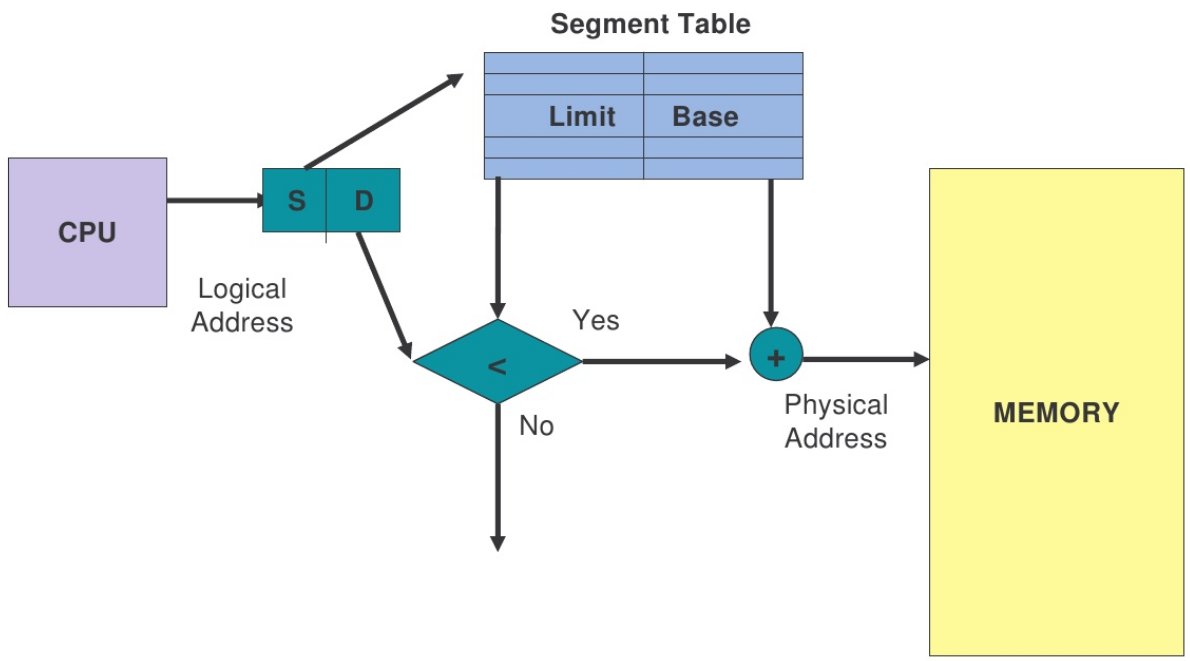
\includegraphics[width=0.8\textwidth]{imgs/memory_segmentation.png}
    \caption{Resolución de una dirección física utilizando un esquema de memoria virtual por segmentos. La segment table en una arquitectura como x86 es ocupada por la GDT o LDT.}
    \label{fig:memory_segmentation}
\end{figure}

\subsection{Paginaci\'on}

La paginaci\'on consiste en dividir la memoria virtual (o l\'ogica) en bloques de un tama\~no fijo (generalmente 4KB) llamados p\'aginas, y la memoria f\'isica en bloques del mismo tama\~no llamados \textbf{frames}. La MMU es la que se encarga de asignar p\'aginas a frames, y las direcciones l\'ogicas est\'an compuestas por una parte que representa el n\'umero de p\'agina, y otra parte que representa el offset dentro de la p\'agina. Es por esto que las p\'aginas siempre deben medir una cantidad de bytes que sean potencias de dos, para poder dividir la direcci\'on en bits de n\'umero de p\'agina y bits de offset.

Las páginas pueden ser guardadas a disco para realizar swapping. Si en el momento de pedir una p\'agina, esta no se encuentra en memoria, se produce una page fault (excepci\'on del sistema operativo), y la rutina de atenci\'on se encarga de cargar la p\'agina en memoria. 

\subsubsection{Tabla de páginas}
Para saber si una p\'agina est\'a en memoria y en qu\'e frame se encuentra, la MMU guarda una tabla de p\'aginas con una entrada por cada p\'agina. En cada entrada entre diversos datos se guarda un bit que indica si la p\'agina est\'a cargada en memoria y el \'indice del frame en el que est\'a cargada. Adem\'as se guardan bits que indican, por ejemplo, si la p\'agina fue modificada luego de ser cargada en memoria, para saber si guardarla en disco al desalojarla o simplemente descartarla y quedarse con la versi\'on que ya hab\'ia en disco. Es importante aclarar que hay una tabla de p\'aginas para cada proceso, es decir, si tenemos $N$ procesos tendremos $N$ tablas de p\'aginas. Esto nos introduce un problema: si por ejemplo tuviésemos 4GB de memoria, y p\'aginas de 4KB, tendr\'iamos una tabla de p\'aginas con un mill\'on de entradas; y esto estaría replicado para cada proceso. 

\subsubsection{Directorio de tablas de páginas}
Se suele dividir las tablas en dos niveles: un directorio de tablas de p\'aginas que apunta a tablas de p\'aginas, a su vez cada una de estas tablas de paginas tendrán en sus entradas las paginas que serán utilizadas por el programa. As\'i, si un proceso usa menos de 4MB de memoria, y las p\'aginas ocupan 4KB, entonces podemos tener un directorio de tablas de p\'aginas con 1024 entradas, una de ellas apuntando a una tabla de p\'aginas con 1024 entradas, y podemos direccionar los 4MB (1024 p\'aginas de 4KB) con tan solo 8KB (4KB del directorio de tablas y 4KB de la \'unica tabla).

\begin{figure}[H]
    \centering
    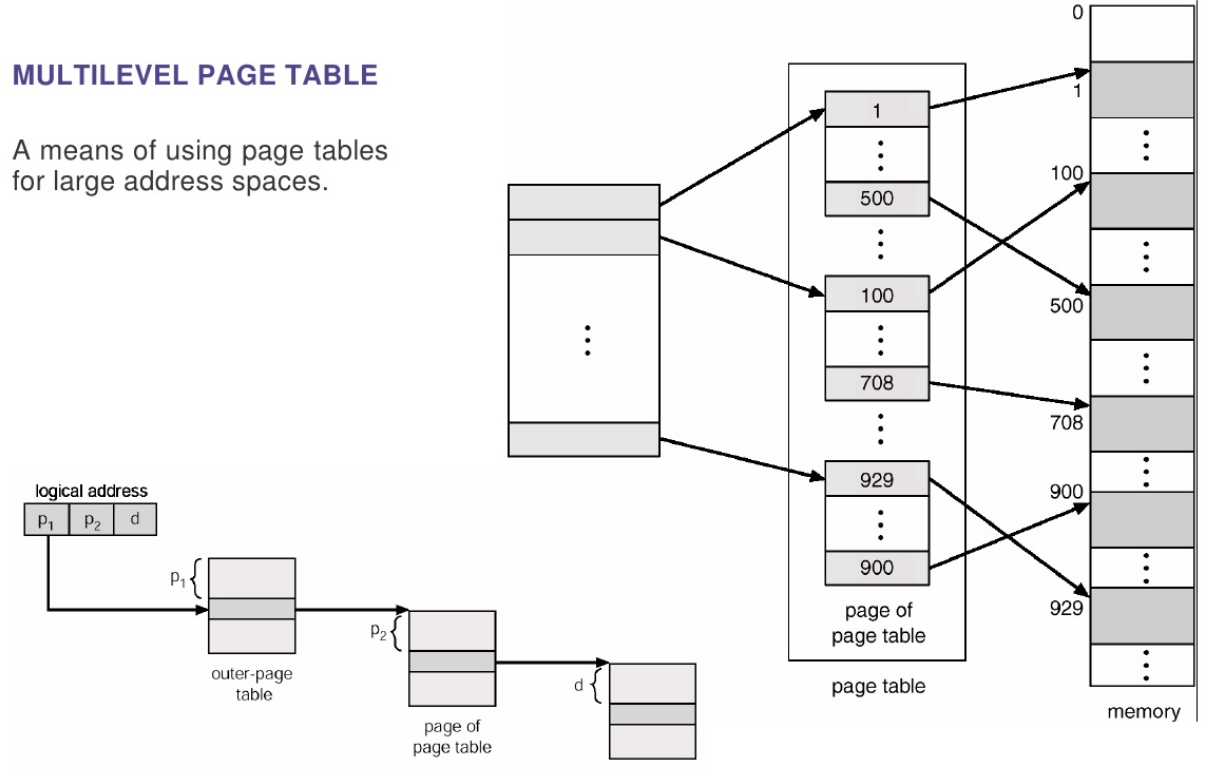
\includegraphics[width=0.8\textwidth]{imgs/memory_multi_level_paging.png}
    \caption{Resolución de una dirección física utilizando paginacion multinivel.}
    \label{fig:memory_multi_level_paging}
\end{figure}

\subsubsection{TLB}
Una de las desventajas de paginaci\'on es que, al tener que convertir las direcciones virtuales en f\'isicas, direccionar una p\'agina puede ser lento, ya que requiere 3 direccionamientos a memoria (directorio, tabla, pagina). Esto en consecuencia hace que obtener instrucciones o datos de la memoria sea m\'as lento. La soluci\'on que se encontr\'o a este problema es una peque\~na cach\'e que se denomina \textbf{Translation Lookaside Buffer (TLB)}. La TLB, tambi\'en conocida como memoria asociativa, contiene el frame en el que se encuentran las p\'aginas m\'as usadas. Al buscar una p\'agina en memoria, lo primero que se hace es buscarla en el TLB, y en caso de que se encuentre presente en el mismo, el acceso a la p\'agina es mucho m\'as r\'apido.

\subsection{Reemplazo de p\'aginas (demand paging)}

Como con paginación todos los bloques son frames del mismo tamaño (el tamaño de las páginas), el problema de decidir en qué bloque de memoria libre cargar una página desaparece. En el caso de que no haya suficiente memoria libre, deberemos utilizar algún algoritmo que decida qué páginas desalojar de memoria. Para todos estos algoritmos existen dos versiones, una donde se desalojan las p\'aginas del mismo proceso (reemplazo local), y otra donde se puede desalojar cualquier p\'agina de memoria (reemplazo global).

Algunos de estos algoritmos pueden ser utilizados como medidas para evitar \textbf{trashing}, es decir, la situación en donde el SO ocupa mas tiempo swapeando páginas que la CPU ejecutando procesos. Esto puede darse cuando la memoria esta llena y hay una alta contención entre los procesos al cargar sus paginas en memoria. Para atenuar los efectos del trashing pueden utilizarse algoritmos de reemplazo local, ya que estos algoritmos obligan al proceso a desalojar sus propias paginas. 

Estudiando mas de cerca los procesos, podremos darnos cuenta que en cada momento un proceso utiliza un determinado subconjunto de páginas de forma intensiva, llamado \textbf{working set}, hasta que en algún punto lo cambia prácticamente en su totalidad. Este comportamiento suele repetirse a lo largo de la ejecución del proceso. Es por esto que los algoritmos de reemplazo local son útiles para atenar los efectos del trashing.

\subsubsection{Algoritmo \'Optimo}

El algoritmo \'optimo de reemplazo de p\'aginas consiste en desalojar de la memoria siempre la p\'agina que va a ser referenciada m\'as tarde, o alguna p\'agina que no vaya a ser nunca m\'as referenciada si existe. Este algoritmo es imposible de implementar pero se utiliza como parámetro de comparación a la hora de medir la performance de otros algoritmos.

\subsubsection{First In First Out}

El algoritmo FIFO consiste en desalojar siempre la p\'agina que fue cargada hace m\'as tiempo entre todas las p\'aginas que est\'an cargadas en memoria, es decir aquella que fue cargada primera. Es uno de los m\'as sencillos pero es bastante ineficiente ya que puede ser que una p\'agina cargada hace mucho tiempo sea una de las m\'as utilizadas.

\subsubsection{Second Chance}

Second Chance es parecido a FIFO, pero difiere en que revisa el bit R de la p\'agina. Si el bit R de la p\'agina m\'as vieja es 0 entonces la desaloja, si en cambio es 1, lo resetea a 0 y la vuelve a encolar como si la p\'agina fuese reci\'en cargada en memoria.

\subsubsection{Clock}

Es muy parecido a Second Chance, pero en vez de guardar una cola, guarda una lista circular, y mueve un puntero a lo largo de la lista. Si una p\'agina tiene el bit R en 1 entonces avanza el puntero a la pr\'oxima posici\'on de la lista. Si encuentra una p\'agina con el bit R en 0, entonces la desaloja y avanza el puntero.

\subsubsection{Least Recently Used}

El algoritmo Least Recently Used desaloja siempre la p\'agina que fue usada hace m\'as tiempo. En vez de guardar el momento en el que fue cargada en memoria, como en FIFO, guarda el momento en el que fue referenciada por \'ultima vez. Dos implementaciones clásicas de este algoritmo son asociando un contador a cada pagina o manteniendo una lista LRU, ambas costosas en términos de hardware ya que se tanto los contadores como la lista tienen que actualizarse en cada escritura y lectura de pagina.


\subsubsection{Not Recently Used}

Las tablas de p\'aginas suelen guardar dos bits R y M que indican si la p\'agina fue referenciada y/o modificada respectivamente desde el momento en el que se carg\'o en memoria. Ambos bits son generalmente seteados por hardware en cada acceso a memoria y el bit R es reseteado peri\'odicamente por el sistema operativo. Las p\'aginas se dividen en cuatro categor\'ias seg\'un los bits R y M:

\begin{enumerate}
\item Ni referenciadas ni modificadas.
\item Modificadas pero no referenciadas (puede pasar cuando el bit R se resetea).
\item Referenciadas pero no modificadas.
\item Referenciadas y modificadas.
\end{enumerate}

El algoritmo Not Recently Used (NRU) desaloja de memoria una p\'agina al azar de la categor\'ia m\'as baja en la que haya al menos una p\'agina. La idea es que las p\'aginas que fueron referenciadas recientemente son m\'as propensas a ser referenciadas nuevamente, y para desempatar, es siempre m\'as costoso desalojar una p\'agina modificada, ya que hay que guardarla a disco.

\subsection{Fragmentación con paginación}

Como vimos anteriormente paginación es un método mucho mas dócil y sencillo que segmentación, por ello es utilizado en los sistemas modernos. Sin embargo, la segmentación no puede ser desactivada en las arquitecturas modernas, por lo que se implementa lo que se llama ``flat segmentation''. Los sistemas operativos modernos solamente definen 4 segmentos: Kernel Code Segment, Kernel Data Segment, User Code Segment y User Data Segment. Esto significa que todos los procesos de usuarios tienen los mismos segmentos de código y datos (por ende, el mismo selector de segmento). Los segmentos solamente cambian cuando se va de usuario a kernel, y se utiliza justamente para diferenciar el espacio de memoria y el modo en el que se esta corriendo (anillo 1 vs anillo 3).

Luego, durante la resolución se resuelve la dirección lineal utilizando la dirección lógica, calculándola utilizando el descriptor de segmento, y luego se resuelve la dirección física utilizando la dirección lineal, utilizando la paginación multinivel.

\begin{figure}[H]
    \centering
    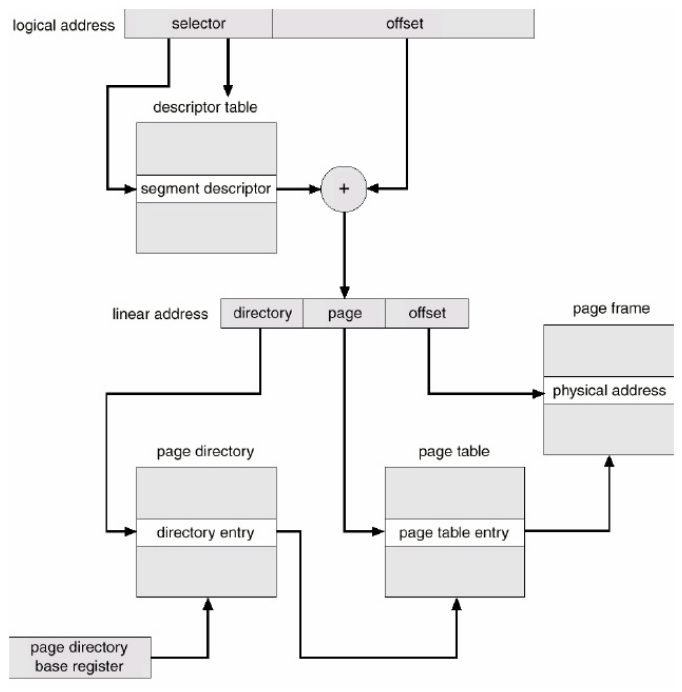
\includegraphics[width=0.6\textwidth]{imgs/memory_paged_segmentation.png}
    \caption{Resolución de una dirección física utilizando fragmentación con paginación multinivel.}
    \label{fig:memory_paged_segmentation}
\end{figure}

\subsection{Copy on Write}

Como vimos anteriormente, un proceso puede crear otros procesos mediante la system call $fork$. Cuando un proceso crea otro proceso, ambos comparten la memoria que ten\'ia el proceso padre. Existen dos opciones para manejar la memoria en este caso: una de ellas consiste en copiar toda la memoria y tener dos copias de los mismos datos y el mismo c\'odigo en memoria desde el principio, y la otra es hacer la copia en alg\'un momento entre que se crea el proceso y se necesita escribir la memoria.

Cuando el sistema operativo decide copiar la memoria al momento en el que uno de los dos proceso decide escribirla, se dice que estamos haciendo Copy on Write.

\section{Protección y seguridad}

En ciertos ambientes académicos los dos términos pueden llegar a tener un significado distinto, sus definiciones formales están dadas por:

La protección se trata de mecanismos para asegurarse de que nadie pueda acceder a los datos del otro (por ejemplo, que un proceso no pueda acceder fuera de su espacio de memoria. También se trata de tener un sistema de autorización que nos permita controlar qué usuario puede hacer cada cosa (por ejemplo, que un proceso no pueda ejecutar cierta parte de la memoria, si no tiene permiso).

La seguridad se trata de asegurarse que quien dice ser cierto usuario, lo sea (por ejemplo, autenticar un usuario en un SO). También se trata de impedir la destrucción o adulteración de los datos.

Sin embargo, en la cátedra no se tendrá en cuenta esta distinción.

\subsection{Seguridad de la información}

En seguridad de la información intentaremos preservar la confidencialidad, integridad y disponibilidad de datos. Para el estudio de estas propiedades es útil tener ciertas abstracciones. Un sistema de seguridad suele tener sujetos, acciones y objetos. La idea es responder: ¿Qué sujetos pueden realizar qué acciones sobre qué objetos?

Como los sujetos, o usuarios, por lo general pertenecen a un grupo (usuarios comunes, administradores, etc), se suelen agrupar en grupos o tener roles. Estos grupos o roles son sujetos del sistema de permisos que nos permite definir la forma de actuar de ciertos sujetos ante ciertos objetos.

\subsubsection{Protocolo AAA}

El protocolo AAA obtiene sus siglas por: Authentication, Authorization y Accounting, que son los pilares fundamentales para cualquier sistema seguro. 

La autentificación nos habla de que una entidad pruebe su identidad ante otra entidad y consiste en la presentación de una propuesta de identidad (por ejemplo un nombre de usuario) y la demostración de credenciales que permiten comprobarla (por ejemplo contraseñas o medios biométricos). La autorización expresa la posibilidad de un sistema de definir qué puede hacer una entidad, en función de su identidad (qué privilegios le doy). Finalmente la contabilidad (accounting), es la habilidad del sistema para dejar registrado que hizo una entidad. El nivel de granularidad de este registro dependerá de forma arbitraria de los que crearon dicho sistema, sin embargo a mayor nivel de granularidad, mas seguro resulta ser el sistema.

\subsection{Autentificación}

En la autentificación de usuarios se utiliza mucho la criptografía ya que, es la rama de la matemática y computación que se ocupa de cifrar/descifrar información utilizando métodos que permitan el intercambio de mensajes de manera que sólo puedan ser leídos por las personas a quienes van dirigidos. De esta manera nos aseguramos que las credenciales de un usuario permanezcan confidenciales.

Por otro lado, también tendremos el criptoanálisis, el cual es el estudio de los métodos que se utilizan para quebrar textos cifrados, con el objeto de recuperar la información original, en ausencia de la clave.

\subsubsection{Funciones de hash}

Son funciones no inversibles que convierten una cadena de caracteres en otra, es decir, que no se puede obtener la pre-imagen (la cadena original) a partir del valor de hash. Son útiles porque, por ejemplo, dado el hash de una contraseña, no queremos que se pueda recuperar la contraseña.

Estas funciones tienen ser resistente a colisiones, es decir que sea difícil encontrar dos elementos distintos cuyo hash sea el mismo (colisión). Porque, por ejemplo, si al autenticarme se verifica el hash de mi contraseña, no quiero que haya otra contraseña distinto cuyo hash sea el mismo.

Las funciones de hash son útiles para almacenar contraseñas, ya que las mismas conviene  guardarlas de modo tal que no se puedan leer, pero estas funciones nos permiten de todas formas comparar una contraseña ingresada con el original almacenado, utilizando la misma función de hash para la contraseña entrante y comparando el resultado. Para asegurar un mayor nivel de seguridad debe usarse salt e iterar la función de hash varias veces. 

Un \textbf{salt} no es mas que una cadena de caracteres que se le agrega a la contraseña para, que en el caso que se quiera ejecutar un ataque de fuerza bruta sobre el hash, no se obtenga la contraseña original. 

Para implementar salt, para cada password p se toma una cadena al azar s (llamada salt). El hash que se almacena es $h(s.p)$ (el de $s$ concatenada con $p$). Como $s$ es aleatorio, $h(s.p)$ es un hash raro que seguro no está en la lista del atacante. No es necesario que la cadena de salt sea secreta, por lo que puede ser almacenada junto con $h(s.p)$. La necesitamos para verificar las contraseñas enviadas por los usuarios. Notar que aún teniendo el $s$ de cada $p$, un atacante no puede ejecutar su ataque tan fácilmente. Ahora, para descifrar una password $p$, tiene que concatenar su salt $s$ a cada password típica $p'$ y verificar si $h(s.p') = h(s.p)$.

Un \textbf{ataque a una función de hash} consiste en probar a lo bruto preimágenes. Si a una password le pasamos $10000$ veces una función de hash (i.e. $h^{10000}(p)$), ahora el atacante para cada prueba tiene que hashear $10000$ veces, lo cual hace que el ataque sea $10000$ veces más lento.

\subsubsection{Algoritmos de encriptación}

Tendremos dos tipos de algoritmos de encriptación: simétricos y asimétricos.

Los algoritmos de encriptación simétricos son aquellos que utilizan la misma clave para encriptar y desencriptar. La clave sólo la deben conocer los extremos de la comunicación. Por ejemplo: Caesar, DES, Blowfish, AES.

Los algoritmos de encriptación asimétricos usan claves distintas. Una de ellas es pública, que puede conocer todo el mundo, y la otra es privada, que sólo conoce el receptor de un mensaje. Por ejemplo: RSA.

\textbf{RSA} es el método de encriptación asimétrica más popular. Produce una clave pública, que puede publicarse, y una privada, que debe mantenerse secreta: $D(E(m, publica), privada) = m$, $D(E(m, privada), publica) = m$. Para mandar un mensaje a una entidad especifica y asegurarse que solo la misma pueda leerlo, se lo encripta usando la clave pública y se manda, la única forma de desencriptarlo luego es utilizando la clave privada. La seguridad de este método se basa en la dificultad para factorizar enteros grandes. El método RSA funciona, a grandes rasgos, de la siguiente manera:

\begin{itemize}
\item Tomemos $p$ y $q$ primos (de 200 dígitos aproximadamente).
\item Multipliquémoslos: $n = pq$.
\item Calculemos también: $n_0 = (p - 1)(q - 1)$.
\item Elijamos un entero e que esté entre $2$ y $n' - 1$ y que sea coprimo (no tener factores comunes) con $n'$.
\item $e$ y $n$ van a ser nuestra clave de encriptación (pública).
\item Computamos d para que cumpla que el resto de $d.e/_0 = 1$.
\item d y n van a ser nuestra clave de desencriptación (privada).
\item \textbf{¿Cómo encripto?} Para cada letra m calculo el resto de dividir $m^e$ por $n$.
\item \textbf{¿Cómo desencripto?} Para cada letra encriptada $c$ calculo el resto de dividir $c^d$ por $n$.
\end{itemize}

Por otro lado, tendremos la \textbf{firma digital con RSA} que se utiliza para asegurarme que un documento es auténtico (que nadie lo cambió). Para obtener una firma digital se calcula el hash del documento que se esta firmando, y se encripta este hash con la clave privada de la entidad que lo firma, luego la firma digital se agrega al documento original. El receptor lo desencripta con la clave pública de la entidad (confiando que la clave pública es efectivamente esa), y si lo puede desencriptar exitosamente, entonces el dueño de la clave pública es efectivamente el autor del documento. Luego, verifica que el hash obtenido de la desencripción se corresponda con el del documento para asegurarse que no se haya alterado.

\subsubsection{Autenticación remota con hash}

La autenticación remota con hash es una forma de autenticación remota de un cliente C en un servidor S. Una posible implementación podría ser la siguiente:
\begin{itemize}
 \item S le manda su clave pública a C para que encripte su password con dicha clave.
 \item C hace lo que S le pide y le manda el resultado.
 \item S desencripta con su clave privada y corrobora la clave de C.
\end{itemize}

Si bien este procedimiento nos brinda cierta seguridad sobre la identidad del cliente, es propenso a un Replay attack: si un atacante M intercepta el mensaje de C a S, entonces M puede autenticarse como C. La solución es utilizar algo llamado Challenge-Response:

\begin{itemize}
 \item Cada vez que C se quiere autenticarse ante S, S elige un número al azar (session token), y se lo manda a C para que encripte su contraseña usando el número al azar como semilla.
 \item C hace lo que S le pide y le manda el resultado.
 \item Ahora a M no le sirve de nada interceptar ese resultado y enviárselo a S para hacerse pasar por C, porque cuando M se comunique con S, S le va a mandar otra semilla.
\end{itemize}

\subsection{Autorización}

\subsubsection{Monitor de Referencias}

El monitor de referencias es el mecanismo responsable de mediar cuando los sujetos intentan realizar operaciones sobre los objetos, se basa en una política de acceso.

La forma más sencilla de concebir a la autorización es como una matriz de control de accesos. La matriz esta compuesta por el producto cartesiano de Sujetos x Objetos, en las celdas figuran las acciones permitidas. Se puede almacenar como una matriz centralizada, o separada por filas o por columnas. Por ejemplo, los archivos suelen guardar sólo lo que puede hacer cada usuario con ellos (es decir, la columna asociada a ese archivo).

Este tipo de representación esta basado en el principio del mínimo privilegio, es decir a cada sujeto sólo permitirle hacer lo mínimo que necesite para funcionar, infiriendo que todo lo que no esta dicho no se puede hacer. Cuando se crea un nuevo objeto se le definen permisos por defecto, que están dados por el tipo de objeto. La matriz también puede ser de Sujetos x (Objetos + Sujetos), puesto que los sujetos también pueden tener permisos sobre cómo actuar sobre otros sujetos.

\subsubsection{DAC y MAC}

El DAC (\textbf{Discretionary Access Control}), es otro esquema de permisos (ACL). La idea bajo este esquema es que los atributos de seguridad se tienen que definir explicitamente por el dueño. Otro esquema posible es \textbf{Mandatory Access Control}, que es utilizado para manejar información altamente sensible. Cada sujeto tiene un grado y los objetos creados heredan el drago del último sujeto que los modificó. La idea es que un sujeto sólo puede acceder a objetos de grado menor o igual que el de él. Un ejemplo de este esquema es Windows Integrity Control, el mismo se basa en el modelo Biba de control de integridad. El mismo define 4 niveles de integridad: System, High, Medium, Low. Los archivos, carpetas, usuarios, procesos, todos tienen niveles de integridad, y el nivel medio es el nivel por defecto para usuarios estándar y objetos sin etiquetas. Un usuario no puede darle a un objeto un nivel de integridad más alto que el suyo.

\subsubsection{DAC en Linux}

El Linux se utiliza DAC, cada archivo tiene un 3 categorías de permisos aplicadas a distintos grupos de sujetos: dueño, grupo y otros. En cada categoría se pueden definir permisos particulares para un grupo de escritura, lectura y ejecución (r, w, x). También tendremos SETUID y SETGID que son permisos de acceso especiales que pueden asignarse a archivos o directorios para permitir a usuarios del sistema ejecutar binarios con privilegios elevados, se denota con s. Se pueden activar estos bits utilizando chmod u<+/->s <archivo> y chmod g<+/->s <archivo>. Todos los usuarios contaran con un id y podrán pertenecer a varios grupos de usuarios, los grupos también contaran con ids.

A veces queremos ejecutar un proceso con mayores privilegios. Por ejemplo para cambiar la contraseña de mi usuario. Queremos ejecutar con los privilegios de root, es decir, del owner del programa. Notar que esta no es una forma de transformar al usuario en root (esto sería un obvio problema de seguridad), sino que sólo estoy ejecutando un programa de root, como root. En definitiva, un proceso tiene dos tipos de uid: el uid del usuario que ejecuta un proceso (uid real) y uid del owner del archivo (uid efectivo). Análogamente para los grupos existe gid real y gid efectivo.

\subsection{Ataques comunes}


En la siguiente sección hablaremos de ataques comunes realizados a protocolos de seguridad.

\subsubsection{Buffer overflow}


Se podría generar overflow en un buffer en stack de una función para cambiar sectores prohibidos de la memoria. Típicamente se usa para cambiar el IP (instruction pointer), que está escrito en la base del stack, también se puede hacer con el heap, llenándolo hasta pisar el IP. La idea es apuntar el IP a una dirección que hayamos llenado del stack con un programa malicioso, de forma tal que al hacer un return el sistema comience a correr esa porción del código utilizando los permisos del programa que estaba corriendo antes

Para evitarlo se pueden hacer chequeos de límites en los accesos a las estructuras de datos (esto es lo que hacen, por ejemplo, Java o C\#), o chequear que no se esté accediendo a sectores prohibidos del stack.

\subsubsection{Control de parámetros}

La idea es pasar un parámetro a un programa, que al ser utilizado genere resultados
inesperados. El caso típico es SQL injection. Hay dos posibles soluciones a este ataque, la primera es utilizar el mínimo privilegio posible y la segunda es validar los parametros. En la practica ambas se utilizan en conjunto.


\subsubsection{Condiciones de carrera}


Una condición de carrera, la cual esta definida como un comportamiento anómalo debido a una dependecia critica inesperada en la temporización de los eventos, puede producir problemas de seguridad. Por ejemplo, una operación que cree un archivo si no existe, puede terminar sobrescribiendo un archivo si las operaciones con las cual se realiza son divisibles.

\subsubsection{Codigo malicioso}

O malware, es software diseñado para llevar a cabo acciones no deseadas y sin el consentimiento explícito del usuario. Algunos tipos de malware pueden incluir:
\begin{itemize}
\item Troyano: es un software que contiene un segmento de código que se aprovecha de su entorno para realizar una acción maliciosa. En otras palabras, malware disfrazado de un programa con otras intenciones.
\item Trap door o backdoor: agujero dejado en un programa a propósito por su creador. Por ejemplo, para que cierto usuario pueda loguearse en un sistema con privilegios máximos.
\item Virus: código embebido en un programa legítimo, que es capaz de replicarse a sí mismo, y que están diseñados para infectar otros programas (modificando o destruyendo archivos).
\item Keylogger: guarda todo lo que se teclea y puede mandarlo via internet a una direccion remota indicada.
\end{itemize}

Las principales vías de infección incluyen: descargas desde páginas web (a veces involuntariamente), adjuntos por email, vulnerabilidades en software, compartir dispositivos de almacenamiento, otros protocolos y aplicaciones de Internet: chat, P2P, redes sociales, etc. Las formas de prevenir estas infecciones es la utilización de antivirus actualizado, recibir las actualizaciones de seguridad debidas para el sistema operativo utilizado, y el uso del sentido común. Sin embargo, aun así en grandes organizaciones siempre hay personas que van a terminar cayendo en estos ataques, y dada la complejidad de una organización, un eslabón pone en peligro la totalidad de la misma. Por eso los administradores de sistemas requieren a soluciones como generadores de claves físicas (o llaves usb) que en conjunto con la contraseña son requeridas para acceder a una cuenta corporativa. Estas claves son la solución definitiva contra ataques de phishing, ya que requieren que la persona inserte físicamente la misma para acceder a una cuenta.

Otras políticas de prevención consisten en denegar la instalación de programas no aprobados por los administradores, sistemas de firewall que deniegan el acceso a sitios previamente aprobados, políticas de acceso a la red interna del trabajo y encriptación de las entradas externas (utilizando VPNs) y registro de las operaciones de cada usuario a recursos compartidos, con tal de poder un análisis pertinente si algo ocurre.

Dentro de desarrollo muchas veces se suele utilizar sandboxing, que es básicamente un mecanismo que provee el SO para aislar procesos, en el caso de linux provee chroot. También suele utilizarse virtualización para tener un sistema totalmente aislado pero con la misma funcionalidad que un sistema operativo completo, en donde se pueden probar diferente tipo de cosas sin riesgo alguno.

\subsubsection{Ataques externos}

Estos ataques están pensados para debilitar las estructuras internas de un sistema y no para tomar control del mismo. Un ejemplo es un ataque DoS (Denial of Service), el mismo consiste en la sobrecarga del ancho de banda de la víctima o de sus recursos computacionales, de forma tal de denegar el acceso a usuarios legítimos. En particular el ataque de acnho de banda es muy difícil de contrarrestar ya que, si es bien ejecutado, no puede ser contrarrestado con software, si no que la forma de contrarrestarlo reside totalmente en la totalidad de ancho de banda que tengamos disponible. Normalmente si poseemos un servicio de hosting para una aplicación, es solucionado por el datacenter que nos provee dicho servicio, mitigando el ataque desde su lado.


Por otro lado un privilege escalation es el aprovechamiento de un bug en un sistema para ganar acceso a recursos que usualmente no son accesibles como usuario.

\subsection{Principios de un sistema seguro}

Los principios generales para un sistema seguro son:
\begin{itemize}
\item Mínimo privilegio.
\item Simplicidad.
\item Validar todos los accesos a los datos.
\item Separación de privilegios.
\item Minimizar la cantidad de mecanismos compartidos.
\item Seguridad multicapa.
\item Facilidad de uso de las medidas de seguridad.
\end{itemize}

En general, cualquier política, mecanismo o procedimiento de seguridad está basado en asumir ciertos hechos. Hay que tener claros cuáles son estos hechos, los cuales normalmente residen en el rol de la confianza. Por ejemplo al bajarnos un parche para solucionar un problema de seguridad del SO confiamos en que el autor del parche es realmente el vendedor del SO y el objetivo del parche realmente es solucionar el problema, y no otro. A veces esto no se cumple y la confianza que los usuarios brindamos a los distribuidores no es respetada. Por eso es que siempre es importante tener en mente que en casos críticos todo esto necesita ser validado.

\section{Sistemas Distribuidos}

Existen tres conceptos que son similares pero no iguales:

\begin{itemize}
\item C\'omputo simult\'aneo (o concurrente): Un scheduler asigna un quantum a cada proceso. Los procesos se ejecutan en una misma CPU de forma concurrente.
\item C\'omputo paralelo: M\'as de una CPU en una misma m\'aquina ejecutando procesos al mismo tiempo. Se suelen compartir el scheduler, clock y memoria en estos tipos de sistemas.
\item C\'omputo distribuido: Varias CPUs ejecutando procesos al mismo tiempo en distintas maquinas, que no comparten fisicamente memoria, clock, etc. Sin embargo en algunos casos la memoria puede ser compartida mediante el modelo de comunacion Linda y el scheduler y clock mediante TTA (Time Triggered Architecture).
\end{itemize}

Las ventajas de tener sistemas distribuidos van desde aprovechar el uso de procesadores en maquinas distintas con el fin de reducir el tiempo de procesamiento; la tolerancia a fallas por la posibilidad de tener replicacion de datos entre maquinas, hasta a veces, en distintas ubicaciones geograficas; y la escalabilidad del sistema, que permite automaticamente contar con mayor cantidad de espacio y poder de computo agregando mas maquinas. Sin embargo, entre las desventajas podremos encontrar la necesidad de lidiar con sincronizacion de procesos, la consistencia de datos y la informacion parcial.

Cuando creamos un sistema distribuido existen limitaciones reales que no permiten gozar de todas las ventajas al mismo tiempo. La Conjetura de Brewer (CAP) examina esta problematica en mas detalle, y nos dice que en un sistema distribuido solo podremos tener dos de tres caracteristicas:
\begin{itemize}
\item Consistencia: todos los nodos ven la misma información al mismo tiempo.
\item Disponibilidad: cada petición a un nodo recibe una respuesta.
\item Tolerancia a partición: sigue funcionando aún si la red falla parcialmente.
\end{itemize}

\subsection{Información parcial}
Una máquina no puede saber todo lo que sucede en el sistema, por lo que se suele dividir el trabajo aplicando paralelismo de datos o paralelismo de tareas. En el paralelismo de datos se aplica el mismo proceso a diferentes datos, por ejemplo paralelizar una multipliacion matricial, mientras que en el paralelismo de tareas se paralelizan distintas tareas, por ejemplo procesando los frames de un video para transmitirlo de forma eficiente via streaming.

\subsection{Comunicacion y Sincronizacion}
Cuando se tiene un sistema distribuido surge la necesidad de sincronizar varias de sus partes, sea bien para realizar un trabajo en conjunto o para comunicar distintas partes de informacion entre los distintos componentes de un sistema.

\subsubsection{Memoria}

Normalmente en los sistemas paralelos se utiliza la memoria para realizar sincronizacion entre procesos. A nivel hardware uno de los modelos mas utilizados es llamado UMA (Uniform Memory Access), el cual centraliza el acceso a memoria desde cada uno de los procesadores por medio de una red de interconexion, esto genera que el acceso a memoria sea igual para cualquier procesador. UMA es normalmente utilizado en cualquier computadora regular con el fin de dar acceso a los distintos CPUs a la memoria RAM. 

\begin{figure}[H]
    \centering
    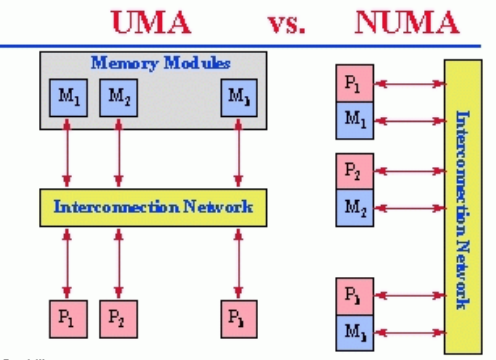
\includegraphics[width=0.5\textwidth]{imgs/numa_uma.png}
    \caption{Modelos UMA y NUMA de memoria.}
    \label{fig:numa_uma}
\end{figure}

Otro modelo utilizado es llamado NUMA (Non-Uniform Memory Access), en donde cada procesador tiene asignada una memoria particular, que puede ser accedida en forma paralela por cada procesador, y una red de interconexion que conecta a los distintos pares de CPU para permitir sincronizacion y consistencia. Este modelo genera que haya areas mas rapidas de acceder que otras para un procesador dado. El mismo es normalmente utilizado con el L1 cache que cada CPU trae asignado, pero tambien puede ser visto en sistemas distribuidos, si consideramos a cada ``CPU'' como una computadora entera.

Por otro lado a nivel software tendremos modelos asociativos estructurados (dado un valor, indican la posicion) y no estructurados, como la memoria virtual global.

\subsubsection{Sincronica}

Este tipo de comunicacion es utilizada por los sistemas de computo distribuidos, en donde muchas veces los modulos del sistema corren en maquinas fisicas distintas. Esto crea la necesidad de poseer protocolos de comunicacion, en este caso sincronica, para el envio de consultas y datos entre los distintos modulos. Dentro de RPC (Remote Procedure Call) sincronico tendremos ejemplos como Java Remote Method Invocation (RMI), JavaScript Object Notation (JSON-RPC) y Simple Object Access Protocol (SOAP), este ultimo construido sobre XML para el envio y recepcion de datos. Este tipo de RPCs luego de enviar una consulta esperan una respuesta en ese momento.

\subsubsection{Asincronica}

Por otro lado tendremos RPCs asincronicos, en donde la respuesta no esta asegurada en el mismo momento en el que se envia la consulta y no se la maneja de dicha manera. Entre algunos de estos tendremos Promises, Futures y Windows Asynchronous RPC, todos estos modelos generan un objeto que tiene una ``promesa'' o la respuesta en un ``futuro'', que una vez obtenida la misma su procesamiento se termina. Son actualmente comunes en frameworks destinados a trabajar con JavaScript, por su modelo de comunicacion asincronica (AJAX).

Tambien existen los sistemas send/receive, que tambien son catalogados como asincronicos. Entre los mismos tendremos el mailbox, pipes no bloqueantes, MPI para C y C++ y Scala actors receive/react.

\subsection{Sistema de archivos}

El sistema de archivos de un sistema distribuido debe poder operar de modo tal que la ubicación física de los archivos sea transparente. Este sistema es el responsable de varias de las ventajas de los sistemas distribuidos como la escalabilidad; que permite almacenar una enorme cantidad de datos, dividiéndolos sobre los discos de muchas máquinas; y la torelancia a fallas; que para asegurarla se suelen implementar replicación y migración. Algunos ejemplos son Hadoop Distributed File System (HDFS) y Red Hat Cluster Storage.

\subsection{Scheduling}

En sistemas distribuidos que comparten procesos entre maquinas y poseen un sistema de scheduling distribuido el mismo se da en dos niveles: local y global. En el \textbf{scheduling local} se le otorga al procesador un proceso ready, esto pasa siempre, en cada round. En el \textbf{scheduling global} se le asigna un proceso a un procesador (mapping).

Dentro del scheduling global se busca compartir la carga entre los distintos procesadores. Para hacerlo existen dos politicas: se puede realizar de manera \textbf{estatica}; en el momento de la creacion del proceso (affinity); o de forma \textbf{dinamica}, en donde la asignacion varia durante la ejecución, llamada tambien migracion (migration).

A la vez la migración puede ser de dos tipos: \textbf{sender initiated} en donde la misma es iniciada por un procesador sobrecargado con el fin de reducir su load; o \textbf{receiver initiated} en donde es iniciada por un procesador libre con el fin de incrementar su load y aprovechar el poder de procesamiento disponible.

En definitiva, la migración es una parte importante de la política de scheduling en sistemas paralelos, y abre otras preguntas: ¿Cuándo hay que migrar un proceso? ¿Qué proceso hay que migrar? ¿A dónde hay que migrarlo? ¿Cómo se difunde el estado?.

\subsection{Comunicacion de mensajes}

\subsubsection{Propiedades}

Requerimientos para una solución de exclusión mutua en sistemas distribuidos:
[EXCL] Exclusión mutua: el recurso sólo lo puede tener un proceso a la vez.
Fairness: las solicitudes de uso deben ser cumplidas en el orden en que fueron hechas.
[LOCK-FREE] Lock-free: el recurso es concedido eventualmente (luego de tiempo finito) a alguno de los procesos que lo solicitó.
[WAIT-FREE] Wait-free: todo proceso que solicita el recurso lo recibe eventualmente.
[G-PROG] Progreso global dependiente: si todo proceso que recibe el recurso lo libera eventualmente, entonces todo proceso que solicita el recurso lo recibe eventualmente.


\begin{itemize}
 \item Exclusion mutua (EXCL): el recurso solo puede ser utilizado por un proceso a la vez.
 \item Progreso (PROG/lock-free):
 \item Progreso global absoluto (wait-free)
 \item Progreso global dependiente (G-PROG/starvation-free)
 \item Justicia (FAIR/fairness)
\end{itemize}

(wait-free es tambien lock-free)




\end{document}










